\documentclass[aps,11pt,twoside,letterpaper]{article}










\usepackage{amsfonts, amssymb, amsmath, amsthm, latexsym}   %, amscd, alltt, setspace, bbm}
\usepackage{epic,eepic}
%\RequirePackage[verbose,
%                letterpaper,
%                top=3cm,
%               left=2cm,
%               right=5cm,
%                bottom=3cm,
%               ]{geometry}
\usepackage{hyperref}


%\usepackage{graphicx}
%\usepackage{xcolor}
%\usepackage{pstricks}               % for figures
%\input{Qcircuit.tex}        % for little circuit diagrams



%MARK STUFF

%\documentclass[smallextended]{svjour3}%
\pdfoutput=1
\usepackage{graphics,amsmath,amsfonts,amscd,revsymb,latexsym,enumerate,multirow,epsfig}
%\usepackage{amsmath}
%\usepackage{amsfonts}
%\usepackage{amssymb}
\usepackage{graphicx}%
\usepackage{fullpage}
\setcounter{MaxMatrixCols}{30}
%TCIDATA{OutputFilter=latex2.dll}
%TCIDATA{Version=5.50.0.2953}
%TCIDATA{LastRevised=Monday, July 20, 2009 02:05:40}
%TCIDATA{<META NAME="GraphicsSave" CONTENT="32">}
%TCIDATA{<META NAME="SaveForMode" CONTENT="1">}
%TCIDATA{BibliographyScheme=BibTeX}
%BeginMSIPreambleData
\providecommand{\U}[1]{\protect\rule{.1in}{.1in}}
%EndMSIPreambleData
\providecommand{\U}[1]{\protect\rule{.1in}{.1in}}



%%% MATH SETS %%%%%%%%%%%%%%
\def\Tr{\textup{Tr}}
\def\c{\mathbb{C}}
\def\z{\mathbb{Z}}
\def\r{\mathbb{R}}
\def\n{\mathbb{N}}
\def\p{\mathbb{P}}
\def\q{\mathbb{Q}}
\def\ph{\varphi}

\def\E{\mathcal{E}}
\def\cH{\mathcal{H}}
\def\NN{\mathbb{N}}


\newcommand{\rhot}{{\ensuremath{\tilde{\rho}}}}
\newcommand{\sigmat}{{\ensuremath{\tilde{\sigma}}}}
\newcommand{\taut}{{\ensuremath{\tilde{\tau}}}}




\hfuzz5pt % Don't bother to report overfull boxes < 5pt


%%% QUANTUM STUFF  %%%%%%%%%%%%%%
\newcommand{\braOket}[3]{\left\langle #1\vert#2\vert#3 \right\rangle}
\newcommand{\e}{  \ensuremath{\mathcal E} }
\newcommand{\x}{  \ensuremath{\mathcal X} }
\newcommand{\m}{  \ensuremath{\mathcal M} }


\renewcommand{\familydefault}{ppl}
\renewcommand{\baselinestretch}{1.0}

% CAPACITY FORMULAS
\newcommand{\ICcap}{  \ensuremath{\mathcal C}_{IC} }
\newcommand{\MACcap}{  \ensuremath{\mathcal C}_{MAC} }
\newcommand{\MMACcap}{  \ensuremath{\mathcal C}_{MMAC} }
\newcommand{\Qcap}{  \ensuremath{\mathcal Q} }
\newcommand{\Ccap}{  \ensuremath{\mathcal C} }
\newcommand{\CcapEA}{  \ensuremath{\mathcal C}_{EA} }
\newcommand{\QcapEA}{  \ensuremath{\mathcal Q}_{EA} }



\newcommand{\mcal}{\mathcal}
\newcommand{\ketbra}[1]{\ket{#1}\bra{#1}}



%%%%%%%%%%%%%%%%%%%%%%%%%%%%%%%%%%%%%%%%%%%%%%%%%%%%%%%%%%%%%%%%%%%%%%%%%%%%%%%%%%%%%%%%%%%%%%%%%%%%%%%%%%%%%%%%%%%%%%%%
%%%%%%%%%%%%%%%%%%%%%%%%%%%%%%%%%%%%%%%%%%%%%%%%%%%%%%%%%%%%%%%%%%%%%%%%%%%%%%%%%%%%%%%%%%%%%%%%%%%%%%%%%%%%%%%%%%%%%%%%
\newtheorem{theorem}{Theorem}
\newtheorem{acknowledgement}[theorem]{Acknowledgement}
\newtheorem{algorithm}[theorem]{Algorithm}
\newtheorem{axiom}[theorem]{Axiom}
\newtheorem{claim}[theorem]{Claim}
\newtheorem{conclusion}[theorem]{Conclusion}
\newtheorem{condition}[theorem]{Condition}
\newtheorem{conjecture}[theorem]{Conjecture}
\newtheorem{corollary}[theorem]{Corollary}
\newtheorem{criterion}[theorem]{Criterion}
\newtheorem{definition}{Definition}
\newtheorem{example}[theorem]{Example}
\newtheorem{exercise}[theorem]{Exercise}
\newtheorem{lemma}{Lemma}
\newtheorem{notation}[theorem]{Notation}
\newtheorem{problem}[theorem]{Problem}
\newtheorem{proposition}[theorem]{Proposition}
\newtheorem{remark}[theorem]{Remark}
\newtheorem{solution}[theorem]{Solution}
\newtheorem{summary}[theorem]{Summary}
%\newcommand{\qed}{{\hfill$\Box$}}
% \newenvironment{proof}{\noindent \textbf{{Proof~} }}{\qed}
\def\bi{\begin{itemize}}
\def\ei{\end{itemize}}
\def\be{\begin{equation}}
\def\ee{\end{equation}}
\def\bea{\begin{eqnarray}}
\def\eea{\end{eqnarray}}
\def\ben{\begin{eqnarray*}}
\def\een{\end{eqnarray*}}
\def\non{\nonumber}
\def\>{\rangle}
\def\<{\langle}
\def\l{\left}
\def\r{\right}
\def\la{\leftarrow}
\def\ra{\rightarrow}
\def\da{{\!\downarrow}}
\def\ot{\otimes}
\def\geqslant{\geq}
\def\leqslant{\leq}
\def\lbL{ \left[\rule{0pt}{2.4ex}\right. }
\def\rbL{ \left.\rule{0pt}{2.4ex}\right] }
\def\lbm{ \left[\rule{0pt}{2.1ex}\right. }
\def\rbm{ \left.\rule{0pt}{2.1ex}\right] }
\def\eps{\epsilon}
\def\g{\gamma}
\def\va{\vec{a}}
\def\vb{\vec{b}}
\def\vx{\vec{x}}
\def\pfail{p_{\text{fail}}}
\def\st{\text{ s.t. }}
\def\bp{{\bf p}}
\def\bq{{\bf q}}
\def\br{{\bf r}}
\def\bH{{\bf H}}
\def\bL{{\bf L}}
\def\bP{{\bf P}}
\def\bQ{{\bf Q}}
\def\bR{{\bf R}}
\def\bS{{\bf S}}
\def\bT{{\bf T}}
\def\bU{{\bf U}}
\def\H{F}
\newcommand{\bA}{{\mathbf A}}
\newcommand{\bB}{{\mathbf B}}
\newcommand{\bE}{{\mathbf E}}
\newcommand{\bG}{{\mathbf G}}
\newcommand{\bI}{{\mathbf I}}
\newcommand{\bX}{{\mathbf X}}
\newcommand{\bY}{{\mathbf Y}}
\newcommand{\bZ}{{\mathbf Z}}
\newcommand{\bN}{{\mathbf N}}
\newcommand{\bu}{{\mathbf u}}
\newcommand{\bv}{{\mathbf v}}
\newcommand{\bx}{{\mathbf x}}
\newcommand{\bz}{{\mathbf z}}
\newcommand{\by}{{\mathbf y}}
\newcommand{\bw}{{\mathbf w}}
\newcommand{\ba}{{\mathbf a}}
\newcommand{\bb}{{\mathbf b}}
\newcommand{\bc}{{\mathbf c}}
\newcommand{\bd}{{\mathbf d}}
\newcommand{\bg}{{\mathbf g}}
\newcommand{\bh}{{\mathbf h}}
\newcommand{\bl}{{\mathbf l}}
\newcommand{\bff}{{\mathbf f}}
\newcommand{\bo}{{\mathbf 0}}
\newcommand{\bee}{{\mathbf e}}
\newcommand{\bal}{{\mathbf \alpha}}
\newcommand{\bbe}{{\mathbf \beta}}
\def\bbC{\mathbb{C}}
\def\bbE{\mathbb{E}}
\def\bbL{{\mathbb{L}}}
\def\bbM{{\mathbb{M}}}
\def\bbN{{\mathbb{N}}}
\def\bbP{{\mathbb{P}}}
\def\bbQ{{\mathbb{Q}}}
\def\bbR{\mathbb{R}}
\def\bbT{\mathbb{T}}
\def\bbZ{\mathbb{Z}}
\def\bbF{\mathbb{F}}
\newcommand{\1} I
\def\one{\openone}
\def\T{{\tt{T}}}
\def\ccG{G}
\def\ccK{K}
\def\cnot{\textsc{cnot}}
\def\dcnot{\textsc{dcnot}}
\def\swap{\textsc{swap}}
\def\UA{U_{\bf A}}
\def\Ucg{U_{\text{CG}}}
\def\Ugpe{U_{\text{GPE}}}
\def\Usch{U_{\text{Sch}}}
\def\Usel{U_{\text{sel}}}
\def\Uqft{U_{\text{QFT}}}
\def\Uxoxo{U_{\text{XOXO}}}
\newcommand{\fig}[1]{Fig.~\ref{fig:#1}}
\newcommand{\eq}[1]{(\ref{eq:#1})}
\newcommand{\peq}[1]{(\ref{eq:#1})}
\newcommand{\eqs}[2]{(\ref{eq:#1}) and (\ref{eq:#2})}
\newcommand{\sect}[1]{Section~\ref{sec:#1}}
\newcommand{\sects}[2]{Sections~\ref{sec:#1} and \ref{sec:#2}}
\newcommand{\thm}[1]{Theorem~\ref{thm:#1}}
\newcommand{\prop}[1]{Prop.~\ref{prop:#1}}
\newcommand{\lem}[1]{Lemma~\ref{lemma:#1}}
\newcommand{\cor}[1]{Corollary~\ref{cor:#1}}
\newcommand{\mscite}[1]{Ref.~\cite{#1}}
\newcommand{\mmcite}[1]{Refs.~\cite{#1}}
\newcommand{\inner}[2]{\langle{#1},{#2}\rangle}
\newcommand{\bra}[1]{\langle #1 |}
\newcommand{\ket}[1]{| #1 \rangle}
\newcommand{\braket}[2]{\langle #1 | #2 \rangle}
\newcommand{\dblbraket}[1]{\mbox{$\langle #1 | #1 \rangle$}}
\newcommand{\proj}[1]{| #1 \>\!\< #1 |}
\newcommand{\oprod}[1]{\l| #1 \r\>\!\!\l\< #1 \r|}
\newcommand{\smfrac}[2]{\mbox{$\frac{#1}{#2}$}}
\newcommand{\upto}[1]{\stackrel{#1}{\approx}}
\newcommand{\rs}[1] {{\rm rowspace} ( #1)}
\newcommand{\iso}[1] {{\rm iso} ( #1)}
\newcommand{\symp}[1] {{\rm symp} ( #1)}
\newcommand{\spann}[1] {{\rm span} \{ #1 \}}
\def\half{\smfrac{1}{2}}
\def\bmath#1{\mbox{\boldmath$#1$}}
\DeclareMathOperator{\diag}{diag} \DeclareMathOperator{\End}{End}
\DeclareMathOperator{\GL}{GL} \DeclareMathOperator{\Hom}{Hom}
\DeclareMathOperator{\id}{id} \DeclareMathOperator{\poly}{poly}
\DeclareMathOperator{\rank}{rank} \DeclareMathOperator{\Sch}{Sch}
\DeclareMathOperator{\sgn}{sgn} \DeclareMathOperator{\Span}{Span}
\DeclareMathOperator{\spec}{spec} \DeclareMathOperator{\tr}{Tr}
\DeclareMathOperator{\vol}{Vol} \DeclareMathOperator{\wt}{wt}
\DeclareMathOperator{\A}{A} \DeclareMathOperator{\B}{B}
\def\HA{\cH_{\A}}
\def\HB{\cH_{\B}}
\def\HAB{\cH_{\A\B}}
\def\*{\star}
\def\ext{\supseteq}
\def\reduction{\stackrel{{}_{\scriptstyle *}}{\geq}}
\def\tilde{\widetilde}
\def\bar{\overline}
\newcommand{\abs}{{\rm abs}}
\newcommand{\rel}{{\rm rel}}
\newcommand{\aux}{{\rm aux}}
\newcommand\app[1]{{\cal A}^{#1}}
\def\cA{{\cal A}}
\def\cB{{\cal B}}
\def\cC{{\cal C}}
\def\cD{{\cal D}}
\def\cE{{\cal E}}
\def\cF{{\cal F}}
\def\cG{{\cal G}}
\def\cH{{\cal H}}
\def\cI{{\cal J}}
\def\cJ{{\cal J}}
\def\cK{{\cal K}}
\def\cL{{\cal L}}
\def\cM{{\cal M}}
\def\cN{{\cal N}}
\def\cO{{\cal O}}
\def\cP{{\cal P}}
\def\cQ{{\cal Q}}
\def\cR{{\cal R}}
\def\cS{{\cal S}}
\def\cT{{\cal T}}
\def\cU{{\cal U}}
\def\cV{{\cal V}}
\def\cW{{\cal W}}
\def\cX{{\cal X}}
\def\cY{{\cal Y}}
\def\cZ{{\cal Z}}
\def\th{\theta}
\def\Th{\Theta}
\def\ga{\gamma}
\def\Ga{\Gamma}
\def\bt{\beta}
\def\al{\alpha}
\def\ep{\epsilon}
\def\vep{\varepsilon}
\def\la{\lambda}
\def\La{\Lambda}
\def\de{\delta}
\def\De{\Delta}
\def\om{\omega}
\def\Om{\Omega}
\def\sig{\sigma}
\def\Sig{\Sigma}
\def\vphi{\varphi}
\def\0{{\mathbf{0}}}
\def\1{{\mathbf{1}}}
\def\2{{\mathbf{2}}}
\def\3{{\mathbf{3}}}
\def\4{{\mathbf{4}}}
\def\5{{\mathbf{5}}}
\def\6{{\mathbf{6}}}
\def\7{{\mathbf{7}}}
\def\8{{\mathbf{8}}}
\def\9{{\mathbf{9}}}
\def\bI{\mathbf{I}}
\def\bb{{\bf b}}
\def\bc{{\bf c}}
\def\bee{{\bf e}}
\def\bl{{\bf l}}
\def\bp{{\bf p}}
\def\bq{{\bf q}}
\def\br{{\bf r}}
\def\bs{{\bf s}}
\def\bt{{\bf t}}
\def\bu{{\bf u}}
\def\bv{{\bf v}}
\def\bw{{\bf w}}
\def\bx{{\bf x}}
\def\by{{\bf y}}
\def\bL{{\bf L}}
\def\bP{{\bf P}}
\def\bK{{\bf K}}
\def\bD{{\bf D}}
\def\bQ{{\bf Q}}
\def\bR{{\bf R}}
\def\bS{{\bf S}}
\def\bT{{\bf T}}
\def\bU{{\bf U}}
\def\fL{\mathfrak{L}}
\def\fl{\mathfrak{l}}
\def\bbC{\mathbb{C}}
\def\bbE{\mathbb{E}}
\def\bbF{\mathbb{F}}
\def\bbG{\mathbb{G}}
\def\bbL{{\mathbb{L}}}
\def\bbM{{\mathbb{M}}}
\def\bbN{{\mathbb{N}}}
\def\bbP{{\mathbb{P}}}
\def\bbQ{{\mathbb{Q}}}
\def\bbR{\mathbb{R}}
\def\bbZ{\mathbb{Z}}
%\smartqed


\hfuzz5pt % Don't bother to report overfull boxes < 5pt





%%% COMMENTS   %%%%%%%%%%%%%%%%%%%%%%%%%%%%%%%%%%%%%%%%%%%%%%%%%%%%%%%%%%%%%%%%%%%%%%%%%%%%%%%%%%%%%%%%%%%%%%%%%%%%%%%%%
\newcommand{\comment}[1]{[\textit{#1}]}


  % header with all macros and Quantum shortcuts




%%%% THEOREMS   %%%%%%%%%%%%%%
%\theoremstyle{plain}
%\newtheorem{Th}{Theorem}[section]
%\newtheorem{Lem}[Th]{Lemma}
%\newtheorem{Prop}[Th]{Proposition}
%\newtheorem{Cor}[Th]{Corollary}
%\theoremstyle{definition}
%\newtheorem{Ex}[Th]{Example}
%\newtheorem{Def}[Th]{Definition}
%\newtheorem{Rem}[Th]{Remark}
%\newtheorem{Quest}[Th]{Question}
%\newtheorem{prf}{Proof}


% CONDITIONAL COMPILATION %%%%%%%%%%%%%%%%%%%%%%%%%%%
\usepackage{ifthen}

% this document has two versions WITHPROOFS is
% intended for Hayden team research group -- without proofs
% is intended for the shorter project version whose page length is bounded above by 8
\newboolean{WITHPROOFS}
\setboolean{WITHPROOFS}{true} % boolvar=true or false






\begin{document}


\title{{\Large Outer bounds on the quantum interference channel} }
\date{\today} 
\author{Ivan Savov \\
    ECSE 612 (multiuser communications) project, McGill University}

%     \email{}
%\affiliation{ School of Computer Science, McGill University, Montreal, Quebec, H3A 2A7, Canada }
%\adress{ECSE 612 (multiuser communications) project, McGill University}
%\keywords{interference channel, quantum Shannon theory, outer bounds}\date{\today }

%%% TODO
% 2/  copy ifdef from multipary mutual independence paper....


\parskip .75ex             % spacing between paragraphs
\maketitle



\begin{abstract}
	In the first part of this work, we present a comprehensive review of
	results about discrete memoryless interference channels.
	In the second part, we define the quantum  multiple access and 
	broadcast channels and state some of the known results about them.
	Finally we attempt to use these MAC and BC results to derive 
	an outer bound on the quantum interference channel. 
\end{abstract}


\section{Introduction}
%%%%%%%%%%%%%%%%%%%%%%%%%%%%%%%%%%%%%%%%%%%%%%%%%%%%%%%%%%%%%%%%%%%%%%%%%%%%%%%%%%%%%%%%%%%%%%%%%%%%%%%%%%%%%%%%%%%%%%%%
%%%%%%%%%%%%%%%%%%%%%%%%%%%%%%%%%%%%%%%%%%%%%%%%%%%%%%%%%%%%%%%%%%%%%%%%%%%%%%%%%%%%%%%%%%%%%%%%%%%%%%%%%%%%%%%%%%%%%%%%


    The interference channel (IC) is a communication network where two transmitters try to send
    information to two receivers using a shared medium. 
    This communication scenario is one of the most general possible in multiuser information
    theory; it includes the multiple access channel (MAC) and the broadcast channel (BC)
    as special cases.
    
    The interference channel is an excellent model for many practical communication scenarios
    where medium contention is an issue. 
    This is why obtaining an expression for the capacity region $\ICcap$ 
    is of central importance to theoretical and practical information theory.
    %
    %was of central interest for theoreticians in the 80s and most recently.
    %
    Despite the numerous efforts, there are very few results about 
    discrete memoryless interference channels (DMIC) known to date.
    Even the special case of Gaussian interference channels there the capacity region is not known.
    % only have for degraded, high interference 
    % the most important case: low / medium interference the capacity is not known...
    

    Recently, quantum information theory (QIT) has been a popular research area in physics,
    computer science and mathematics. This new field of information theory is firmly based
    in Shannon's principle of information-as-statistics, but systems that behave 
    according to the laws of quantum mechanics.
    The current state of QIT is similar to that of classical information theory in the 80s,
    when most single user problems had been solved and researchers were exploring new
    grounds in multiuser information theory.
    It is therefore an appropriate time to study the quantum interference channel.

    
    This paper will try to review classic results on the interference channel and
    define the problem in the quantum setting.
    %Specifically we will try to focus on the 
    In section \ref{Preliminaries} we will define the basic concepts related to
    the classical interference channels.
    Then in section \ref{section:lit-review} we will reproduce the main results
    from a series of seminal classical papers on the interference channel.
    Results relating to outer bounds on the IC capacity are collected together
    in section  \ref{section:outer-bounds}.
    The following section (section \ref{section:quantum}) deals with the quantum generalization of the
    multiple access and broadcast channels. 
    	In order to make this work more self-contained, we have included
	in appendix \ref{section:intro_to_qit} a detailed introduction to 
	the ideas of quantum information theory.  Readers not familiar with quantum information theory are encouraged 
    to consult appendix \ref{section:intro_to_qit} before diving reading section \ref{section:quantum}.
    Finally we have a section of discussion and pointers to open problems in section  \ref{section:discussion}.

    
    
    
 \section{Preliminaries}  \label{Preliminaries} 

    In this section we introduce important notation and nomenclature which will
    be used throughout this paper.
    We also state some important results from multiuser information theory,
    which we will need as building blocks.

    \subsection{Definitions}
	
        \begin{definition}[Interference network]
            A two party interference network $(\cX_1 \otimes \cX_2, p(y_1,y_2|x_1,x_2), \cY_1 \otimes \cY_2)$ 
            is general model for communication networks with two inputs, two outputs and a probability transition
            matrix $p(y_1,y_2|x_1,x_2)$.
        \end{definition}
        

        \begin{definition}[Interference channel]
            A two party interference channel is a particular use of an interference network 
            $(\cX_1 \otimes \cX_2, p(y_1,y_2|x_1,x_2), \cY_1 \otimes \cY_2)$ 
            where messages $M_1,M_2$ are independently encoded into a codewords $X_1,X_2$ 
            at rates $(R_1,R_2)$ with $Y_1,Y_2$ being the intended receiver.
        \end{definition}

        \begin{definition}[Achievable rate pair]   \label{def:achievableICrates}
            We say that a rate $(R_1,R_2)$ is achievable for a channel 
            $(\cX_1 \otimes \cX_2, p(y_1,y_2|x_1,x_2), \cY_1 \otimes \cY_2)$
            if there exists a code for $n$ uses of the channel where the messages 
            taken from respective sets $\{1,2,\ldots,2^{nR_1} \}$ and
             $\{1,2,\ldots,2^{nR_2} \}$ are transmitted with vanishing error probability
             \be
             	\Pr\left\{ M_1 \neq \hat{M}_1 \text{ or }  M_2 \neq \hat{M}_2 \right\} \leq \epsilon.
		\label{eqn:ICerrors}
             \ee
        \end{definition}
        
        \begin{definition}[Capacity]
            The capacity region $\ICcap$ of is the convex hull of the closure of the set of achievable rate pairs $(R_1,R_2)$.
        \end{definition}


        \begin{definition}[Degraded channel] \label{def:degraded-channel}
            Let $Y \sim p_y(y|x_1,x_2)$ and $Z \sim p_z(z|x_1,x_2)$ be two random variables 
            defined in terms of $X_1,X_2$.
            %
            We say $Y$ is a \emph{degraded version} of $Z$ with respect to $(X_1,X_2)$ if
            there exits $Y'$, defined on the same sample space as $Y$, such that 
            $p_{y'}(y'|x_1,x_2,z)=p_{y'}(y'|z)$ and $p_{y'}(y'|x_1,x_2) = p_y(y|x_1,x_2)$.
        \end{definition}
        
        Another way to say the above is that $Y'$ is statistically equivalent to $Y$ and
        that $(X_1,X_2) \to Z \to Y' $ form a Markov chain.
        

    \subsection{Convex sets, closures and optimization constraints}
    	
	Rate regions in multiuser information theory often stated in terms of constrained 
	optimization problems over information theoretic quantities.
	Furthermore, because of the \emph{time-sharing} principle, 
	we can achieve any rate in the \emph{convex hull} of any other achievable rates.
	
	To rigorously state each capacity result can become overly wordy if we do not
	find a compact notation to express the above notions.
	Luckily, smarter people than us have already found such a compact notation \cite{Sato77}.
	We illustrate it with a well known result \cite{S48}.
	
	The classical capacity of a single user channel $(\cX,p(y|x),\cY)$ is given by
	\be
		\mathcal{C} = \operatorname{conv} \bigcup_{p(x)} \{ R  \ | \ R \leq I(X;Y) \  \} .
	\ee
	Where the $p(x)$ which we are optimizing over should not be confused with 
	the $p(y|x)$ associated with the channel.
	The $\operatorname{conv}$ is not really necessary in this case.
	
	Technically speaking, the rate $R = I(X;Y)$ is not achievable for the single user channel,
	but any rate $R-\epsilon$ is.
	The rigorous way of saying this would be to refer to ``the closure of'' the set or rates 
	$R < I(X;Y)$, but we will avoid this extra mathematical  kung fu and simply use equalities 
	$R \leq I(X;Y)$ for our rate constraints.


    \subsection{Multiple access channel} \label{subseciton:MAC}

        The multiple access channel (MAC) is a special case of the interference channel with a single 
        receiver. 
        It is therefore important to review briefly the known capacity result for the MAC.

        \begin{definition}[MAC]
            A multiple access channel is defined as $(\cX_1 \otimes \cX_2, p(y|x_1,x_2), \cY)$,
            and models a communication network with two inputs and one output with 
            the probability transition matrix $p(y|x_1,x_2)$.
        \end{definition}
        
        The MAC channel is one of the few problems multiuser information theory for which
        we know precisely the capacity region.
        \be
                \MACcap  = \operatorname{conv} \bigcup_{p(x_1)p(x_2)} 
                		\{ (R_1,R_2) | \text{ Eqn. \eqref{Gmac1} } \}  \label{region:G_MAC}
        \ee
        \bea
            R_1         &\leq&      I(X_1;Y|X_2), \nonumber \\
            R_2         &\leq&      I(X_2;Y|X_1), \label{Gmac1} \\
            R_1 +R_2    &\leq&      I(X_1X_2;Y). \nonumber
        \eea 

	The coding strategy that makes these rates possible is \emph{successive decoding}.
	The receiver first decodes one of the two messages, then decodes the second
	message using the first as side information. 
	The better rate is obtained for the second message, since we have side information.
	Note that the rates $R_1=I(X_1;Y|X_2)$ and $R_2=I(X_2;Y|X_1)$ are not simultaneously
	achievable.

    \subsection{Broadcast channel}
        
        While the capacity of the broadcast channel (BC) is not known in general,
        there are several insights learned from BCs that also apply to the
        study of interference channels.
        
        The first thing to note is that the error criterion in equation \eqref{eqn:ICerrors}
        of definition \ref{def:achievableICrates} only depends on the marginals 
        $p_1(y_1|x_1x_2)$ and $p_2(y_2|x_1x_2)$.
        This is because if we manage to get both decoding errors low,
        then we manage to get the error of the union of the two events also.
        
        This observation leads us to the fact that all channels which have
        the same marginals will have the same capacity. More formally, we will define
        the class $K(p)$ of interference channel probability matrices 
        that have the same marginals as $p(y_1,y_2|x_1x_2)$:
        \be
 		\label{eqn:Kp}
        		K(p) \triangleq \{ q(y_1,y_2|x_1,x_2) \  \big| \ q_1(y_1|x_1,x_2) = p_1(y_1|x_1,x_2), \ 
					q_2(y_2|x_1,x_2) = p_2(y_2|x_1,x_2) \}.
        \ee
        
        Thus the capacity region $\ICcap$ for an IC channel with probability transition matrix $p$, is the 
        same for all channels in $K(p)$.
        In particular, we can define a particular member of $K(p)$ which might be simpler to analyse
        \begin{definition}[Independent channel]
            Let $p_1(y_1|x_1,x_2)$ and $p_2(y_2|x_1,x_2)$ be the marginals of the associated
            with some interference network $p(y_1,y_2|x_1,x_2)$.
            We define the \emph{independent channel} the interference network with 
            product probability transition matrix
            \be
                p_i(y_1,y_2|x_1,x_2) = p_1(y_1|x_1x_2)p_2(y_2|x_1x_2).
            \ee
        \end{definition}


    \subsection{Other uses of the interference network}

        The interference channel is not the most general communication scenario
        that we can consider using the the interference network.
        One possibility is to require transmitters to send messages to both
        receivers.
	%        , which will make the channel more similar to a multiple-broadcast
	%        channel.
	%
        Another generalization % that we will not be considered here is
        of the IC problem is to allow for correlations between the channel inputs $X_1,X_2$.
        To study this problem we must also be familiar with Slepian-Wolf
        coding of correlated sources. 
	%
        We will briefly mention these and other generalization of the IC in the discussion
        section (section  \ref{section:discussion}) at the end of this document.

        




%%%%%%%%%%%%%%%%%%%%%%%%%%%%%%%%%%%%%%%%%%%%%%%%%%%%%%%%%%%%%%%%%%%%%%%%%%%%%%%%%%%%%%%%%%%%%%%%%%%%%%%%%%%%%%%%%%%%%%%%
%%%%%%%%%%%%%%%%%%%%%%%%%%%%%%%%%%%%%%%%%%%%%%%%%%%%%%%%%%%%%%%%%%%%%%%%%%%%%%%%%%%%%%%%%%%%%%%%%%%%%%%%%%%%%%%%%%%%%%%%
\section{Classical results on the Interference Channel}   \label{section:lit-review}

    
    In this section we present a literature review of important papers 
    on the interference channel.
    

%    \subsection{Early papers}


        \subsection{Ahlswede 74: The capacity region of a channel with two senders and two receivers} \ \\
        
            One of the earliest papers to appear on the topic of interference channels is by Rudolf Ahlswede \cite{Ahlswede1974}.
            While the notions of entropy and mutual information were already well established in those days, 
            the notation had not yet been standardized so the author uses the definitions of entropic 
            quantities from first principles like this one
            \be
                R_1(p,q,Y_1) \triangleq
                    \sum_{x_1, x_2, y_1} 
                        p(x_1)q(x_2)p(y_1|x_1,x_2) 
                        \log \frac{ p(y_1|x_1,x_2) }{ \sum_{x_1} p(x_1)p(y_1|x_1,x_2) },
            \ee
            which stands for $I(X_1;Y_1|X_2)$ in modern notation.

            The paper defines three communication problems that can be studied on the
            interference network $p(y_1,y_2|x_1,x_2)$. 

            \begin{itemize}
                \item   The {\bf MAC}  to receiver $Y_1$ with probability
                	    distribution is $\sum_{y_2} p(y_1,y_2|x_1,x_2)$.
                        Ahlswede calls this the $(p,T_{21},I)$ \emph{communication situation}.

                \item   The {\bf IC} problem which we have defined above. In Ahlswede's nomenclature
                        this is a  $(p,T_{22},I)$ communication situation.

                \item   Finally there is the {\bf multiple MAC} (MMAC)  problem, where 
                        messages $M_1$ and $M_2$ are to be decoded at both receivers.
                        This is called the  $(p,T_{22},II)$  problem in the paper.

            \end{itemize}

            The first result in this paper is an alternate proof  of the $Y_1$-{MAC} capacity region.
            We already stated capacity region $\MACcap$ in subsection \ref{subseciton:MAC}.
            

            The author then uses the same arguments to prove the capacity of the MMAC channel
            when the two inputs $X_1$ and $X_2$ are allowed to be correlated.

            \be
                    C_{MMAC}  = \operatorname{conv} \bigcup_{p(x_1,x_2)} \{ (R_1,R_2) | \text{ Eqn. \eqref{Gmmac} } \} 
            \ee
            \bea
                R_1         &\leq&      \min\{ I(X_1;Y_1|X_2), I(X_1;Y_2|X_2) \}, \nonumber  \\
                R_2         &\leq&      \min\{ I(X_2;Y_1|X_1), I(X_2;Y_2|X_1) \}, \label{Gmmac} \\
                R_1 +R_2    &\leq&      \min\{ I(X_1X_2;Y_1), I(X_1X_2;Y_2) \} \nonumber 
            \eea 
            
            Note that the optimization is done over joint distributions $p(x_1,x_2)$ and thus
            does not quite fit into the paradigm of independent messages which we 
            are interested in.
		%
            Indeed, the author  makes a remark in the conclusion of the paper, that knowing the 
            capacity of the MMAC problem does not help us directly to find the capacity of the IC channel.
                        
	%	            \comment{ Why need correlated sources? } \\
	%            Let $\mathcal{R}_{p(x_1,x_2)}$ be the closure \comment{of the convex hull?} of rates $(R_1,R_2)$ which
	%            satisfy equations  \eqref{r1-in-mmac-thm} through \eqref{r1-in-mmac-thm}.
	%            And let $\mathcal{C}(p,T_{22},II)$ be the capacity of for the MMAC problem with correlated sources.
	%            We want to show that $\mathcal{R}_{p(x_1,x_2)} = \mathcal{C}(p,T_{22},II)$.

	%

	%            \comment{ Is there an intuitive explanation why this is true? } \\
	%            For the part $\mathcal{R}_{p(x_1,x_2)} \subseteq \mathcal{C}(p,T_{22},II)$ we have the following argument...
	%            if you have some rates $R_1$ and $R_2$ that are feasibly for both the $Y_1$-MAC and the $Y_2$-MAC then
	%            you must be able to do the MMAC problem too.
            
	%            The other direction $\mathcal{R}_{p(x_1,x_2)} \supseteq \mathcal{C}(p,T_{22},II)$  




        \subsection{Sato 77: Two-user communication channels} \ \\

            Perhaps the most important of the early papers on the interference channel is 
            by Hiroshi Sato \cite{Sato77}.
            In this paper the IC problem is defined and the relations between it and the
            MAC and BC are outlined.
            
            Using these relations, the author proves a several progressively stronger 
            outer bounds the best of which is presented in equation \eqref{region:Gsato} in
            the next section.
            
            % negative result using twin channel...
            
            This paper is where degraded IC make their first appearance.
            The author gives an inner bound $G_D$ for the degraded IC,
            but this bound is not equal to the outer bound.
            The Sato outer bound and the inner bound $G_D$ do coincide,
            however, for a special case of degraded channels called \emph{twin channels}.
            

        \subsection{Carleial 78: Interference channels} \ \\

            The paper by Carleial is yet another comprehensive discussion 
            on interference channels \cite{Carleial78}. 
            This paper proves the naive outer bound on the IC (see equation \eqref{Gnaive} below),
            and the Sato outer bound \eqref{region:Gsato} which is  better
            because of the sum rate inequality.

            The author also proves an inner bound counterpart to the naive outer bound, 
            which we will call the naive inner bound
	        \be
	        		\label{GnaiveINNER}
	        		G_{ach}  \triangleq \left\{ (R_1,R_2) \in \operatorname{conv}  \{ P_1, P_2, O \}   \right\},
	        \ee
	        where the three points are defined as 
	        \bea \label{eqn:naive-bound}
	            P_1      &=&    (I(X_1;Y_2|X_2),\ 0), \nonumber \\
	            P_2     &=&     (0, \ I(X_2;Y_2|X_1)), \nonumber \\
	            O     &=&     (0,0). \nonumber 
	        \eea            
	   \begin{theorem}[Theorem 1 in \cite{Carleial78}]
	   	The capacity region $\ICcap$ satisfies $G_{ach}  \subseteq \ICcap$.
	   \end{theorem}
	   \begin{proof}
		Consider the $Y_1$-MAC sub-channel of the IC.
		We know from the result on the MAC channel (equation \eqref{region:G_MAC}) 
		that the rate $R_1 = I(X_1;Y_2|X_2)$ is achievable for the $Y_1$-MAC. 
		Thus the point $P_1~=~(I(X_1;Y_2|X_2),\ 0)$ is achievable for the IC.
		%
		A similar argument is applied to show $P_2$ is achievable 
		using the $Y_2$-MAC sub-channel. By the time sharing principle,
		we can achieve any rate in the convex hull of these points.
	   \end{proof}
            
            Carleial also generalizes the notion of  \emph{twin channels} which he calls
            ``interference channels with statistically equivalent outputs'' for which he 
            calculates the capacity region. 
            These channels are simple to analyze because both receivers $Y_1$ and $Y_2$
            obtain the same information and thus the IC problem reduces to the MAC problem.

            Using his result on the twin channel he gives loose inner and outer bounds for  
            degraded ICs. To get an inner bound, he creates a twin channel from the 
            degraded channel by discarding part of the information at the better receiver.
            To obtain the outer bound, he uses the reasoning that all degraded outputs
            have less information than the best channel output, thus the capacity of the
            twin channel with copies of the best output forms an outer bound on the degraded IC capacity.
            
            The paper then discusses some examples: binary ICs and Gaussian ICs.
            Even for these simplistic examples of ICs we cannot calculate the capacity region.
            %
            In the section dealing with Gaussian ICs, the author sows the seeds of two
            important ideas which would later be taken up by others and proven for general ICs.
            The first of these ideas is the notion of successive decoding which would be
            later be used by Han and Kobayashi for the general DMIC \cite{HK81}.
            The second idea is the notion of channels with \emph{strong interference} where the 
            interference in the channel is so bad that it is easier for a receiver to decode the interfering
            message (intended for the other receiver) than the one intended for him.
            
        
    \subsection{Han-Kobayashi / Cheng-Motani-Garg inner bound}


        The best achievable region for the interference channel is due to Han and Kobayashi \cite{HK81}.
        By splitting the message $M_1$ intended for Rx1 into public and personal parts, 
        $M_{10}$ and $M_{11}$ respectively and using successive  decoding at the receivers
        we can achieve a rate region $G_{HK}$ described by 14 inequalities.
        
        Recently Cheng, Motani and Garg simplified the H-K coding strategy and relaxed some 
        of the decoding requirements in order to obtain a simpler achievable rate region where the rates
        are bounded by only 7 inequalities \cite{CMGE08}.
        A further contribution by Han and Kobayashi shows that the two regions are in fact 
        equivalent \cite{kobayashi2007further}.
        
        Without further ado, we present the HK-CMG rate region, which we will call this way to give credit to all.
        \be
        		G_{HK}  = G_{CMG} \triangleq \operatorname{conv} 
		\bigcup_{p(x_1|u_1)p(x_2|u_2)p(u_1)p(u_2)} \{ (R_1,R_2) | \text{ Eqn. \eqref{Rcmg} } \} 
        \ee
        \bea
            R_1 		&\le&	I(X_1;Y_1| U_2 ) \nonumber \\
            R_2 		&\le&	I(X_2;Y_2| U_1 ) \nonumber \\
            R_1 + R_2	&\le&	I(X_1U_2; Y_1) + I (X_2; Y_2|U_1U_2) \nonumber \\
            R_1 + R_2	&\le&	I (X_1; Y_1|U_1U_2) + I (X_2U_1; Y_2) \label{Rcmg}\\
            R_1 + R_2	&\le&	I (X_1U_2; Y_1|U_1) + I(X_2U_1; Y_2|U_2) \nonumber  \\
            2R_1 + R_2	&\le&	I (X_1U_2; Y_1) + I (X_1; Y_1|U_1U_2) + I(X_2U_1;Y_2|U_2) \nonumber \\
            R_1 + 2R_2	&\le&	I (X_2; Y_2|U_1U_2) + I (X_2U_1; Y_2) +  I (X_1U_2; Y_1|U_1) \nonumber 
        \eea
        
        
%	\subseciton{Other papers}
%	
%		We


%%%%%%%%%%%%%%%%%%%%%%%%%%%%%%%%%%%%%%%%%%%%%%%%%%%%%%%%%%%%%%%%%%%%%%%%%%%%%%%%%%%%%%%%%%%%%%%%%%%%%%%%%%%%%%%%%%%%%%%%
%%%%%%%%%%%%%%%%%%%%%%%%%%%%%%%%%%%%%%%%%%%%%%%%%%%%%%%%%%%%%%%%%%%%%%%%%%%%%%%%%%%%%%%%%%%%%%%%%%%%%%%%%%%%%%%%%%%%%%%%
\section{Outer bounds on $\mcal{C}_{IC}$}           \label{section:outer-bounds}

    In this section we present the best known outer bounds on the IC capacity region $\mcal{C}_{IC}$.
    
    \subsection{Naive bound}
        
        The first bound, comes from the relationship to the multiple access channel.
        In particular we can think of the interference channel as two separate MACs -- one with $Y_1$ as output
        and another one with $Y_2$ as output.
        The probability distributions for these MACs are $p(y_1|x_1,x_2) = \sum_{y_2} p(y_1,y_2|x_1,x_2)$ and 
        $p(y_2|x_1,x_2) = \sum_{y_1} p(y_1,y_2|x_1,x_2)$ respectively.

        Note that if some rate $R_1$ is achievable for the IC, then it must also be achievable for 
        the $Y_1$-MAC channel since it is a special case of the IC. 
        %
        We define the following ``rectangle'' region:
        \be
        		\label{Gnaive}
        		G_{Naive}  \triangleq \operatorname{conv} 
			\bigcup_{p(x_1)p(x_2)} \{ (R_1,R_2) | \text{ Eqn. \eqref{eqnsGnaive} } \}  
        \ee
        \bea \label{eqn:naive-bound}
            R_1     &\leq&    I(X_1;Y_2|X_2), \nonumber \\
            R_2     &\leq&    I(X_2;Y_2|X_1). \label{eqnsGnaive}
        \eea
        
        The region defined above forms our first outer bound on the IC rate region.
        \begin{theorem}
             The region $G_{Naive}$ defined in \eqref{Gnaive} is an outer bound on $\ICcap$, i.e.
             \be
                \ICcap \subset G_{Naive}.
            \ee
        \end{theorem}
        \begin{proof}
            Suppose, for contradiction, that some rate $R^*_1 > I(X_1;Y_2|X_2)$ is achievable for the IC.
            As pointed out above, this means that it must also be achievable for the $Y_1$-MAC channel.

            But we know from equation \eqref{region:G_MAC} the exact capacity region for the MAC channel,
            and rate $R^*_1$ lies clearly outside of that region, so it must not have been achievable 
            for the IC in the first place.
		%
            A similar argument is applied for the second inequality using the $Y_2$-MAC sub-channel.
        \end{proof}        
         
        This bound is in general very loose. Note however that this bound is achievable
        for an IC that is independent, i.e. one with probability distribution
        \be
            p(y_1,y_2|x_1,x_2) = p_i(y_1,y_2|x_1,x_2) = p(y_1|x_1,x_2)p(y_2|x_1,x_2).
        \ee


        
    \subsection{Sato's BC bound}
        
        We can describe a more precise outer bound to the capacity region by specifying
        an inequality on the sum rate $R_1+R_2$. 
        This was done by Hiroshi Sato \cite{Sato77} by adapting his results on the 
        broadcast channel \cite{Sato1978}.
        
        Consider a IC with probability transition matrix $p(y_1,y_2|x_1,x_2)$, 
        we define the Sato region associated with that channel as follows.
        \be
        		G_{Sato}(p)  \triangleq \operatorname{conv} \bigcup_{p(x_1)p(x_2)} \{ (R_1,R_2) | \text{ Eqn. \eqref{Gsato} } \} 
		\label{region:Gsato}
        \ee
        \bea \label{eqn:sato-outer-bound}
            R_1             &\leq&    I(X_1;Y_1|X_2),  \nonumber \\
            R_2             &\leq&    I(X_2;Y_2|X_1),  \label{Gsato} \\
            R_1+R_2    &\leq&    I(X_1X_2;Y_1Y_2). \nonumber 
        \eea
        
        We now state two adaptations of the BC capacity outer bounds which apply directly 
        to the interference channel.
                
        \begin{theorem}[Theorem 1 in \cite{Sato77}]
             The region $G_{Sato}$ defined in \eqref{region:Gsato} is an outer bound on $\ICcap$, i.e.
             \be
                \ICcap \subset G_{Sato}(p).
            \ee
        \end{theorem}        
        \begin{proof}
        		To obtain the first two inequalities, we use the same argument as in the proof of
		$G_{Naive}$.
		The third inequality follows from the consideration of a MAC channel
		where the output is $Y=(Y_1,Y_2)$ which gives us the bound
		$R_1+R_2 \leq I(X_1X_2;Y)$.
		
		Combining the two outputs $Y_1$ and $Y_2$ is equivalent to allowing 
		joint decoding for the interference channel.
		Since the joint-decoding channel is more powerful than the original IC,
		any outer bound on the joint-decoding IC is also an outer bound on $\ICcap$.
        \end{proof}        
        
        Furthermore, using the fact that the IC capacity $\ICcap$ is the same for all channels 
        in the same-marginals class $K(p)$ defined in equation \eqref{eqn:Kp}, we can take
        the intersection of $G_{Sato}$ over all channels in that class.
        
        \begin{theorem}[Theorem 2 in \cite{Sato77}]
             \be
                \ICcap \subset \bigcap_{q \in K(p)} G_{Sato}(q).
            \ee
        \end{theorem}        
        \begin{proof}
            The IC capacity is the same for all channels in $K(p)$, so we might as well
            pick the worst case in $K(p)$, which is exactly what the intersection operation accomplishes.
        \end{proof}        
        


    \subsection{Carleial}

        A further development concerning an outer bound was obtained by Carleial \cite{Carleial83}.
        
        Consider the two random variables $Z_1,Z_2$ such that 
        \bea
            Y_1 &\textrm{ is a degraded version of }& Z_1, \\
            Y_2 &\textrm{ is a degraded version of }& Z_2, \\        
            Y_2 &\textrm{ is a degraded version of }& (X_1,Z_1), \\        
            Y_1 &\textrm{ is a degraded version of }& (X_2,Z_2),
        \eea
        
	%        If we think of $Z_1,Z_2$ as the outputs of the channel, we can interpret the above
	%        conditions as the following. 
	%        Knowing the input and output of the other person's communication we can recover our own signal.
	%        %
	%        If we manage to decode our message correctly, then I can also simulate the output that the other
	%        person has received -- i.e. I have a joint decoder on $(Y_1,Y_2)$.
	%        
        
        then we have the following outer bound
        \be
        		G_{Carl}  \triangleq \operatorname{conv} \cup_{p(x_1)p(x_2)} \{ (R_1,R_2) | \text{ Eqn. \eqref{Gcarl} } \} 
        \ee
        \bea
            R_1             &\leq&    I(X_1;Y_1|X_2)  \nonumber \\
            R_2             &\leq&    I(X_2;Y_2|X_1)   \label{Gcarl}\\
            R_1+R_2     &\leq&   \min\!\left\{ \ I(X_1X_2;Z_1) \ , \ I(X_1X_2;Z_2) \ \right\}             \nonumber 
            %R_1+R_2     &\leq&   I(X_1X_2;Z_1) \\
            %R_1+R_2     &\leq&    I(X_1X_2;Z_2) 
        \eea
        
        This bound can be shown to be strictly tighter than the Sato bound and is the best known outer bound
        on the interference channel.
        
        
        
	%    \subsection{Nair - El Gamal outer bound}
	%       
	%        \comment{is this useful?}
	%        
	%        In a recent paper \cite{Nair2006}, Nair and El Gamal give the following outer bound on the BC
	%        with independent messages $M_1,M_2$ encoded into $U,V$ respectively,
	%        which are later \emph{jointly encoded} into an input symbol $X$ for the BC.
	%        
	%        \bea \label{eqn:nair-outer-bound}
	%            R_1             &\leq&    I(U;Y_1) \\
	%            R_2             &\leq&    I(V;Y_2) \\
	%            R_1+R_2     &\leq&   I(U;Y_1) + I(V;Y_2 | U) \\
	%            R_1+R_2     &\leq&   I(V;Y_2) + I(U;Y_1 | V) 
	%        \eea        
	%        for some choice of input distribution $p(u,v,x)=p(u,v)p(x|u,v)$. 
	%        
	%        The region defined above is an outer bound on the BC, which
	%        involves joint encoding of the two sources $U,V$.
	%        If we are dealing with the IC, we have a more restrictive scenario
	%        since $U \to X_1$ and $V \to X_2$, i.e. we don't have joint encoding
	%        of the two sources.
	%        
	%        It follows that the above region is also an outer bound on the IC cap region.
	%        




%%%%%%%%%%%%%%%%%%%%%%%%%%%%%%%%%%%%%%%%%%%%%%%%%%%%%%%%%%%%%%%%%%%%%%%%%%%%%%%%%%%%%%%%%%%%%%%%%%%%%%%%%%%%%%%%%%%%%%%%
%%%%%%%%%%%%%%%%%%%%%%%%%%%%%%%%%%%%%%%%%%%%%%%%%%%%%%%%%%%%%%%%%%%%%%%%%%%%%%%%%%%%%%%%%%%%%%%%%%%%%%%%%%%%%%%%%%%%%%%%
\section{Quantum multiuser information theory}      \label{section:quantum}

	Quantum information theory (QIT) has been an area of very active research in the past decade.
	Ever since B. Schumacher's discovery that quantum information can be compressed 
	just like its classical counterpart \cite{Sc95},
	information theorists and physicists have been working hard to answer the basic questions
	about source coding, channel capacity and efficient coding schemes for quantum system.
	
	QIT can be considered in some sense a direct extension of classical information theory.
	It is not surprising then if many QIT results carry the same flavour as the classical counterpart.
	Often times, the rates obtained in a quantum protocol will be bounded by the same expressions 
	in terms of mutual information as in the classical result (up to a constant factor of $\frac{1}{2}$).
	
	This resemblance at the ``formula level'' is misleading, however, since very often the equations
	come about for very different reasons.
	Indeed, the properties of quantum information and the von Neumann entropy used
	to measure it, have some very different characteristics compared to classical information.
	
	Here is a short list with a few of the particularities quantum information has to offer:
	
	\begin{itemize}
		\item 	Quantum information cannot be copied. This is called the \emph{no-cloning} principle.
		\item 	Quantum information cannot be destroyed. A quantum system only ``loses'' 
				information in the sense that it gets mixed up in the environment. 
				This is in fact not strictly a quantum property, even classical laws of physics are 
				reversible at the micro-level.
		\item 	Entanglement can be used to increase the rates of certain protocols despite being
				provably useless as a communication resource by itself (no-signalling principle from Special Relativity).
				(classically shared randomness cannot increase the rate of IT protocols)
		\item 	von Neumann conditional entropy can be negative,
				$H(A|B)_\rho < 0$, and this has an operational interpretation related to quantum Slepian-Wolf coding.
		\item 	Monogamy of entanglement:  If we have some tripartite pure state on $ABC$,
				then the more entangled $A$ is with $B$, the less entangled it can be with $C$.
		%	and we
		%	can prove that the $A$-entanglement is not in system $B$, then it must be in system $C$ 
		%	because it must be somewhere.
		%				If a pure system $\ket{\psi}^{ABR}$ is such that 
		%				the $A$ and $B$ subsystems are in a tensor product state $\psi_{AB}=\psi^{A}\otimes \psi^{B}$,
		%				then the ``quantum information'' contained 
		\item		Polygamy of purification: In a pure tripartite state on $ABC$, some subset $\hat{B} \subsetneq B $ can,
				with hight probability, contain the purification of two \emph{both} $A$ and $C$.
		\item		Quantum Error Correcting Codes exist. 
				Despite the fact that quantum information is in some sense continuous,
				we can still \emph{stabilize} it using a finite set of operations just like classical ECC.
	\end{itemize}	

	For a crash-course introduction to the subject, and in particular the notation
	used the reader can consult Appendix A at this point.
	For a more in depth introduction to the subject an excellent book is \cite{NC04}.


	In this section we will review some of the known results in quantum information theory
	that about the multiple access and broadcast channels. 
	Before we get to that, we must discuss the kinds of rates that one might want to study.


	\subsection{Communication tasks}
			
		We can use a quantum channel to transmit classical or quantum information.
		There are therefore two different communication tasks and different capacity regions
		associated with each task for the same quantum channel $\mathcal{N}$.
		To complicate things further, we often consider coding strategies, which use an additional
		communication resource of shared entanglement  between sender	and receiver.
		
		Thus, there are 4 different capacities:
		\begin{itemize}
			\item Classical data: $\mathcal{C}\!\left(\mathcal{N}\right)$ \vspace{-0.1in}
			\item Quantum data: $\mathcal{Q}\!\left(\mathcal{N}\right)$ \vspace{-0.1in}
			\item Entanglement-assisted classical data: $\mathcal{C}_{\texttt{E-A}}\!\left(\mathcal{N}\right)$ \vspace{-0.1in}
			\item Entanglement-assisted quantum data: $\mathcal{Q}_{\texttt{E-A}}\!\left(\mathcal{N}\right)$
		\end{itemize}
	
		Suppose we have coding strategy that makes $n$ uses of the channel $\mathcal{N}$.
		A common but not universal convention is to denote rates for the communication
		of classical information by the letter $R$ (number of bits sent per channel use),
		and the quantum rates by the letter $Q$. 
		Quantum rates measure the dimension of the system $\psi$ that we managed
		to send across the channel so $Q=\frac{1}{n}\log \dim \psi$.
		In cases where we do not consider entanglement to be ``free'', we will 
		denote by $E$ the rate at which entanglement is being used-up or generated
		by the protocol.
		
		
	\subsection{Quantum multiple access channels}
	

		 A quantum multiple access channel is a map $\mcal{M}^{A'B' \to C}$ that
		 takes two quantum systems as inputs and produces a third quantum system.
		 
		 
		 The quantum MAC was first studied in  \cite{huang2000classical}, 
		 where the authors investigated the classical capacity.
		 The authors, however, studied the classical capacity in 
		 a paradigm in which allows for correlations between the quantum states
		 input to the channel. This approach is similar to Ahlswede's correlated input approach
		 to the MMAC problem \cite{Ahlswede1974}.
		
		
		 The classical capacity  $\mathcal{C}_{QMAC}\!\left(\mathcal{M}\right)$ of the quantum MAC
		 was not proven until one year later by Winter  \cite{winter2001capacity}.
		 
		\begin{theorem}[Theorem 10 in \cite{winter2001capacity}]
		The capacity of the quantum MAC $\mcal{M}$ to carry classical information is 
		$\mcal{C}_{QMAC}(\mcal{M}) = \frac{1}{n} \bigcup_{n=1}^\infty \mcal{C}^{(1)}_{QMAC}(\mcal{M}^{\otimes n})$ where 
	        \be
	        		\mcal{C}^{(1)}_{QMAC}  = \operatorname{conv} 
				\bigcup_{p(x_1)p(x_2)\sigma_{x_1}\sigma_{x_2}} 
				\{ (R_1,R_2) | \text{ Eqn. \eqref{qGmac1} } \}  \label{region:qG_MAC}
	        \ee
	        \bea
	            R_1         &\leq&      I(A;C|B)_\theta, \nonumber \\
	            R_2         &\leq&      I(B;C|A)_\theta, \label{qGmac1} \\
	            R_1 +R_2    &\leq&      I(AB;C)_\theta, \nonumber
	        \eea 
	        where mutual informations are calculated with respect to 
		\be
			\theta = \sum_x p(x_1)p(x_2) \ketbra{x_1}_A \otimes 
					\ketbra{x_2}_B \otimes \mcal{M}\!({\sigma_{x_1}} \otimes \sigma_{x_2} )_C.
		\ee
		\end{theorem}    
		This paper by Winter is also interesting for our purposes because it is the only place
		in literature where the quantum interference channel is mentioned.
		The author mentions that he is not sure how to extend his coding strategy to the
		case of multiple decoders. 
		

		The next set of contributions on the quantum MAC problem are by Yard et al  \cite{Yard2008} 
		and the conference version \cite{yard2005capacity}.
		In these papers, the authors give regularized capacity regions for the 
		classical-quantum capacity region  $\mathcal{CQ}(\mcal{M})$, where one of the inputs
		to the MAC is classical and the other is quantum.
		
		The authors also give a multi-letter formula for $\mathcal{Q}(\mcal{M})$, 
		the quantum capacity region for the MAC.
		\begin{theorem}[Theorem 2 in \cite{yard2005capacity}]
			The capacity of the quantum MAC $\mcal{M}^{A'B' \to C}$ to carry quantum information is 
			$\mcal{Q}_{QMAC}(\mcal{M}) = \frac{1}{n} 
				\bigcup_{n=1}^\infty \mcal{Q}^{(1)}_{QMAC}(\mcal{M}^{\otimes n})$ where 
		        \be
		        		\mcal{Q}^{(1)}_{QMAC}  = \operatorname{conv} 
					\bigcup_{p(x_1)p(x_2)\sigma_{x_1}\sigma_{x_2}} 
					\{ (Q_1,Q_2) | \text{ Eqn. \eqref{q2Gmac1} } \}  \label{region:q2G_MAC}
		        \ee
		        \bea
		            Q_1         &\leq&      I_c(A \rangle BC)_\omega, \nonumber \\
		            Q_2         &\leq&      I_c(B \rangle AC)_\omega, \label{q2Gmac1} \\
		            Q_1 +Q_2    &\leq&      I_c(AB \rangle C)_\omega, \nonumber
		        \eea 
		        where mutual informations are calculated with respect to the state 
			\be
				\omega^{ABC} =  \id^{AB}\otimes\mcal{M}\!(\Psi_1 \otimes \Psi_2 ),
			\ee
			and the states $\ket{\Psi_1}^{AA'}$ and $\ket{\Psi_1}^{BB'}$ are pure.
		\end{theorem}    
		
		
		
		\bigskip
		
		Recently, the entanglement assisted capacity of the QMAC channel was proved by
		Hsieh, Devetak and Winter in \cite{Hsieh2008}.
		
		
		\begin{theorem}[Theorem 2 in \cite{Hsieh2008}]
			Consider the quantum MAC $\mcal{M}^{A'B' \to C}$. For some states $\rho^{A'}_1$
			and $\rho^{B'}_2$ define the output of the channel 
			\be
				\theta^{ABC} = \id^{AB}\otimes\mcal{M}(\varphi_1^{AA'} \otimes \varphi_1^{BB'}  ),
			\ee
			where $\ket{\varphi_1}^{AA'}$ and $\ket{\varphi_1}^{BB'}$ are purifications of $\rho^{A'}_1$
			and $\rho^{B'}_2$ respectively.
			Define the two dimensional region 
		        \be
		        		\mcal{C}_{\texttt{E-A}}^{(1)}(\mcal{M})  = \operatorname{conv} \bigcup_{\rho_1, \rho_2 }
					 \{ (R_1,R_2) | \text{ Eqn. \eqref{qGmac2} } \}  \label{region:G_MAC1}
		        \ee
		        \bea
		            R_1         &\leq&      I(A;C|B)_\theta, \nonumber \\
		            R_2         &\leq&      I(B;C|A)_\theta, \label{qGmac2} \\
		            R_1 +R_2    &\leq&      I(AB;C)_\theta. \nonumber
		        \eea 
		        Then the entanglement-assisted capacity region $\mcal{C}_{\texttt{E-A}}(\mcal{M})$
		        is given by the regularized expression 
		        \be
		        		\mcal{C}_{\texttt{E-A}}(\mcal{M}) = 
					\overline{ 
						\bigcup_{n=1}^\infty \mcal{C}_{\texttt{E-A}}^{(1)}(\mcal{M}^{\otimes n}) 
						}.
		        \ee
		\end{theorem}    
	
		% single letter for sum rate 
		
		Note that by using the teleportation protocol we can obtain the quantum 
		entanglement assisted rate region $\mcal{Q}_{\texttt{E-A}}(\mcal{M})$ 
		which will be of the same form but each of the inequalities in \eqref{qGmac2}
		will have a $\frac{1}{2}$ in front of it.
		
		
		
		

		

	\subsection{Quantum broadcast channels}


		The quantum BC problem has received comparatively little attention.
		The problems with the quantum BC are not only technical (proving theorems), 
		but also conceptual (defining the problem).
		The classical broadcast problem defines three rates. 
		Two personal rates  $R_1,R_2$ for messages intended for Rx1, Rx2 respectively
		and a rate $R_0$ for message $M_0$ recoverable at both receivers.

		In the quantum BC, we can define rates $Q_1,Q_2$ in analogy with their
		classical counterparts but since we are not allowed to copy quantum information,
		how could we possibly deliver a common quantum message $\ket{M_0}$ to both receivers?
		%
		This problem of not being able to copy quantum information is not
		unique in the BC case. 
		In the study of quantum network coding, it is equally difficult to find a 
		quantum analog of the multicast scenario which requires a common message
		to to be delivered to multiple receivers.
		
		%	Thus it is not surprising then, if researchers choose to consider only 
		%	the personal rates $Q_1,Q_2$ and mixed situations where some of the
		%	broadcast information is classical.
		
		The first result on the quantum BC is by Yard, Hayden and Devetak \cite{YHD2006}.
		They define three problems and prove a multi-letter capacity region for each of them.
		The first of these problems involves a special kind of channel that does not 
		really fit well with the rest of QIT. This channel as a classical input and a quantum output.
		
		The second result concerns the classical-quantum capacity $\mathcal{CQ}(\mcal{N})$
		for a quantum channel $\mcal{N}^{A' \to BC}$ where the sender (Alice) wants to 
		send quantum information to Rx1 (Bob) at a rate $Q$ while at the same time 
		broadcasting a common message $M_0 \in \{ 1, 2, \ldots, 2^{nR_0} \}$ to both receivers.
		The authors give a proof of a multi-letter capacity region for this problem.
		%		The rates that are achievable are
		%		\bea
		%			Q 	&\leq&	\frac{1}{n} I(A \rangle B^nT)_\sigma,  \\
		%			R_0	&\leq&	\frac{1}{n} \min \{  I(T; B^n)_\sigma,\ I(T; C^n)_\sigma \}, 
		%		\eea
		%		where the mutual informations are taken with respect to
		%		\be
		%			\sigma^{TAB^nC^n}	=	\bigoplus_t p(t)\mcal{N}^{\otimes n}\!\!\left( \phi_t^{A'^{n}} \right)^{B^nC^n},
		%		\ee
		%		which is the outcome of $n$-copies of the channel applied to the $A'$ part 
		%		of some ensemble $\{p(t),\ \ket{\phi_t}^{AA'} \ \}$.
		
		The third result of that paper considers a true quantum broadcast scenario.
		In order to circumvent the difficulties of copying quantum information outlined above,
		the authors give a protocol which establishes GHZ states of the form
		\be
			\ket{GHZ}^{ABC}	=		\frac{1}{\sqrt{2}} \left( \ket{000}^{ABC} + \ket{111}^{ABC} \right),
		\ee
		which are a form of tripartite entanglement.
		At a later point in time, this communication resource can be used 
		to establish quantum  communication between any two of three parties users.
		Thus, generating this GHZ is equivalent to being able to communicate
		with either of the two receivers (but not both) and we can decide whom
		we wish to communicate with later on.
		
		
		\bigskip
		The second (and better) paper on the quantum broadcast channel is by 
		Dupuis\footnote{Fr\'ed\'eric Dupuis used to sit just across the room from me until last summer.} 
		and Hayden \cite{DH2006}.
		In this paper the authors reproduce the classical Marton achievable rates 
		for the entanglement assisted quantum capacity $\mathcal{Q}_{\texttt{E-A}}\!\left(\mathcal{N}\right)$.
		
		\begin{theorem}[Theorem 2 in \cite{DH2006}]
			Let $\mcal{N}^{A' \to B_1B_2}$ be a quantum broadcast channel. 
			Then the following rate region is achievable for 
			$\ket{\psi}^{A_1A_2B_1B_2DE} = U_{\mcal{N}}^{A' \to B_1B_2E}\ket{\phi}^{A_1A_2A'D}$,
			where $\ket{\phi}$ is any pure state:
			\bea
				Q_1 	&\leq&	\frac{1}{2} I(A_1; B_1)_\psi,  \nonumber \\
				Q_2	&\leq&	\frac{1}{2} I(A_2; B_2)_\psi,  \\ 
			Q_1+Q_2	&\leq&	\frac{1}{2} \left[ I(A_1; B_1)_\psi + I(A_2; B_2)_\psi - I(A_1; A_2)_\psi \right].  \nonumber
			\eea			
			$Q_1$ is the rate at which Alice sends qubits to Bob 1, and likewise $Q_2$ for Bob 2.
		\end{theorem}
		
		The authors also prove a multi-letter converse for the same rate region
		and also show how this result can be adapted to give an inner bound
		for the quantum capacity $\mathcal{Q}\!\left(\mathcal{N}\right)$ without 
		entanglement assistance.
		

		


	
	\subsection{Quantum interference channel}

		
		In this section we will define clearly the quantum interference channel problem.
		The quantum IC is an open problem in quantum information theory and has
		not been attempted yet. 
		Hopefully, this project will be the first setting stone in that direction.
		
		\begin{definition}
			The quantum interference network $\mathcal{N}^{A_{1}^{\prime}A_{2}^{\prime}\rightarrow B_{1}B_{2}}$
			is a completely-positive trace-preserving map that takes two quantum inputs 
			and produces two quantum outputs.
		\end{definition}
		
		\begin{definition}
			The quantum interference channel problem with entanglement assistance 
			is a particular use of the interference network 
			$\mathcal{N}^{A_{1}^{\prime}A_{2}^{\prime}\rightarrow B_{1}B_{2}}$ such
			that two independent quantum states $\psi^{A_1},\psi^{A_2}$ 
			are transmitted faithfully to their respective receiver at rates $(Q_1,Q_2)$,
			possibly using entanglement between sender and receiver in the process.
		\end{definition}
		
		We will now outline a general protocol for entanglement-assisted
		transmission of quantum information over the quantum interference network
		$\mathcal{N}^{A_{1}^{\prime}A_{2}^{\prime}\rightarrow B_{1}B_{2}}$. 
		%
		Two spatially separated senders control the respective input systems
		$A_{1}^{\prime}$ and $A_{2}^{\prime}$, and two spatially separated receivers
		will be given the respective output systems $B_{1}$ and $B_{2}$. 
		%
		The channel has an	extension to an isometry $U_{\mathcal{N}}^{A_{1}^{\prime}A_{2}^{\prime
		}\rightarrow B_{1}B_{2}E}$, where $E$ models the environment.
		%
		The task of sender $i$ is to transmit a $2^{nQ_{i}}$-dimensional quantum
		system by exploiting some large number $n$ uses of the channel $\mathcal{N}$
		and entanglement in the form of $2^{nE_{i}}$ ebits shared with receiver $i$,
		where $i\in\left\{  1,2\right\}  $. The goal for receiver $i$ is to decode
		with high fidelity the quantum state that sender $i$ transmits.

		An $(n,Q_{1},Q_{2},\epsilon)$ \textit{entanglement-assisted quantum
		interference channel code} (EAQIC) can be described in five steps: the inputs,
		the encoding, the transmission, decoding and the error analysis.
		We detail each of these steps below.
		
		\begin{enumerate}

		\item {\bf Input.} 
		Each sender given the quantum state which is to be sent in register
		$A_{i}$ alongside an auxiliary register $T_{A_{i}}$ that contains the entanglement shared
		with receiver $i$. Let $R_{i}$ be a quantum register that contains the
		purification of the state in register $A_{i}$. The overall input state is%
		\[
		\psi^{R_{1}A_{1}}\otimes\Phi^{T_{A_{1}}T_{B_{1}}}\otimes\psi^{R_{2}A_{2}%
		}\otimes\Phi^{T_{A_{2}}T_{B_{2}}}.
		\]

		\item \textbf{Encoding.} 
		Sender $i$\ encodes the registers $A_{i}$ and
		$T_{A_{i}}$ according to some CPTP\ encoding map $\mathcal{E}_{i}%
		^{A_{i}T_{A_{i}}\rightarrow A_{i}^{\prime}}$. The state after the encoding
		maps is%
		\[
		\sigma^{R_{i}A_{i}^{\prime n}T_{B_{i}}}\equiv\mathcal{E}_{i}^{A_{i}T_{A_{i}%
		}\rightarrow A_{i}^{\prime}}(\psi^{R_{i}A_{i}}\otimes\Phi^{T_{A_{i}}T_{B_{i}}%
		}).
		\]
		The overall state after encoding is%
		\[
		\rho^{R_{1}A_{1}^{\prime n}T_{B_{1}}R_{2}A_{2}^{\prime n}T_{B_{2}}}%
		\equiv\sigma^{R_{1}A_{1}^{\prime n}T_{B_{1}}}\otimes\sigma^{R_{2}A_{2}^{\prime
		n}T_{B_{2}}}.
		\]
		Observe that the state between $R_{1}A_{1}^{\prime n}T_{B_{1}}$ and
		$R_{2}A_{2}^{\prime n}T_{B_{2}}$ is a product state.

		\item \textbf{Transmission.} 
		Both senders input their respective systems
		$A_{1}^{\prime n}$ and $A_{2}^{\prime n}$ into the quantum
		interference channel $\mathcal{N}^{A_{1}^{\prime n}A_{2}^{\prime n}\rightarrow
		B_{1}^{n}B_{2}^{n}}$. The resulting state is%
		\[
		\omega^{R_{1}B_{1}^{n}T_{B_{1}}R_{2}B_{2}^{n}T_{B_{2}}}\equiv\mathcal{N}%
		^{A_{1}^{\prime n}A_{2}^{\prime n}\rightarrow B_{1}^{n}B_{2}^{n}}(\rho
		^{R_{1}A_{1}^{\prime n}T_{B_{1}}R_{2}A_{2}^{\prime n}T_{B_{2}}}).
		\]
		Observe that the state between registers $R_{1}B_{1}^{n}T_{B_{1}}$ and
		$R_{2}B_{2}^{n}T_{B_{2}}$ is not necessarily a product state.

		\item \textbf{Decoding.} The two receivers obtain the respective systems
		$B_{1}^{n}$ and $B_{2}^{n}$ from the output of the channel. Receiver $i$
		performs a CPTP\ decoding map $\mathcal{D}_{i}^{B_{i}^{n}T_{B_{i}}%
		\rightarrow\hat{A}_{i}}$ that combines the channel output $B_{i}^{n}$ with his
		half $T_{B_{i}}$ of the entanglement shared with sender $i$. The state after
		these decoding maps is%
		\[
		\theta^{R_{1}\hat{A}_{1}R_{2}\hat{A}_{2}}\equiv(\mathcal{D}_{1}^{B_{1}%
		^{n}T_{B_{1}}\rightarrow\hat{A}_{1}}\otimes\mathcal{D}_{2}^{B_{2}^{n}T_{B_{2}%
		}\rightarrow\hat{A}_{2}})(\omega^{R_{1}B_{1}^{n}T_{B_{1}}R_{2}B_{2}%
		^{n}T_{B_{2}}}).
		\]
		
		
		\item {\bf Error analysis.} 
		The conditions for a good quantum code are that both receivers be
		 able to decode the quantum states from the
		respective senders with high fidelity:%
		\[
		F\left( \theta^{R_{1}\hat{A}_{1}R_{2}\hat{A}_{2}}, \  
			\psi^{R_{1}A_{1}}\otimes\psi^{R_{2}A_{2}} \right) \geq 1- \epsilon.
		\]
		
		\end{enumerate}
		
		Figure~\ref{fig:interference-protocol}\ depicts all of the above steps as
		they would occur in any entanglement-assisted quantum interference channel code.
		\begin{figure}[hptb]
		\begin{center}
		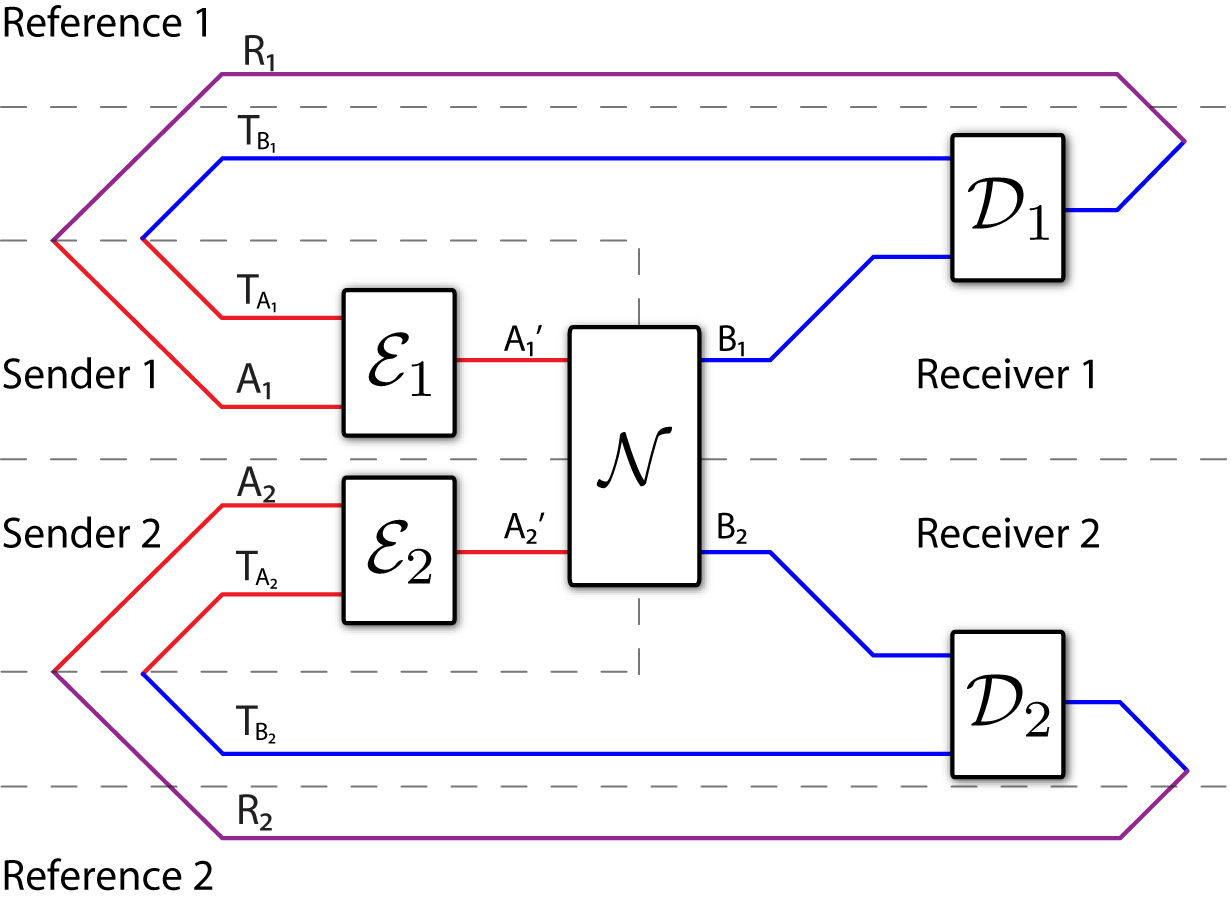
\includegraphics[width=5in]{interference-protocol.png}
		\caption{The circuit diagram for an entanglement-assisted quantum interference
		channel code. }%
		\label{fig:interference-protocol}%
		\end{center}
		\end{figure}
		%EndExpansion

		
		\begin{definition}
			A rate pair $(Q_{1},Q_{2})$ is \textit{achievable} if there exists an
			$(n,Q_{1}-\delta,Q_{2}-\delta,\epsilon)$ entanglement-assisted quantum
			interference channel code for any $\epsilon,\delta>0$ and sufficiently large
			$n$.
		\end{definition}

		\begin{definition}
			The capacity region
			$\mathcal{C}^{QIC}_{\texttt{E-A}}\!\left(\mathcal{N}\right)$
			is the closure of the set of all achievable rates $(Q_{1},Q_{2})$.
		\end{definition}



%		Now that we have all the formalities out of the way




		

		
%%%%%%%%%%%%%%%%%%%%%%%%%%%%%%%%%%%%%%%%%%%%%%%%%%%%%%%%%%%%%%%%%%%%%%%%%%%%%%%%%%%%%%%%%%%%%%%%%%%%%%%%%%%%%%%%%%%%%%%%
%%%%%%%%%%%%%%%%%%%%%%%%%%%%%%%%%%%%%%%%%%%%%%%%%%%%%%%%%%%%%%%%%%%%%%%%%%%%%%%%%%%%%%%%%%%%%%%%%%%%%%%%%%%%%%%%%%%%%%%%
\section{Discussion and conclusion}		\label{section:discussion}

    In this section we will make reference to some of the generalizations and open problems
    associated with the study of interference channels.
    
    


    What is the most general use of the interference network we can think of?
    The most general classical problem to consider involves six indpendent
    messages: 3 starting at Tx1 and 3 starting at Tx2 with rates
    \be
    	\vec{R}	=	( R_{11}, R_{12}, R_{10},  \ R_{21}, R_{22}, R_{20} ),
    \ee
    where $R_{ij}$ ($i,j \in \{1,2\}$) is the rate for the message from sender $i$
    to receiver $j$ and $R_{k0}$ ($k \in \{1,2\}$) is a broadcast rate from sender $k$
    to both receivers.
    %
    The interference channel problem cuts out the two dimensional $R_{11}$, $R_{22}$ plane
    and ignores all the remaining rates.
    The MMAC problem cuts out the $(R_{10}, R_{20})$  two dimensional region.
    
        Are these cross rates not useful? 
        These extra rates could maybe be converted into some other information resource.
        In the classical case, these extra messages could be used for some cooperative 
        behaviour. 
	In the quantum case, with the addition of entanglement between receivers they 
	could perhaps be used with some post-processing to improve the direct
	transmission rates $R_{11}$, $R_{22}$.
        I feel these cross rates should be taken into account in general.

        
        % correlated sources
        As mentioned several times in this paper, there exists an even more general
        model for the MAC and the IC in which the inputs are allowed to be correlated.
        %
        I think that understanding joint source-channel coding in the multiuser case
        is a very interesting problem. Some early work on the subject \cite{cover1980multiple},
        reveal that it depends on a polymatroid structure which is very interesting
        since it connects with deeper notions about polytopes \cite{E69, poly}.
        

        The capacity of the classical interference channel remains an open problem.
        Furthermore we have added the new problem of finding the capacity of the
        quantum interference channel. Which problem will be solved first?

	The fact that after so many years we still don't know $\ICcap$ begs 
	an even more fundamental question. 
	Are the techniques of information theory general enough to study such problem?
	Perhaps an even more pressing question for quantum information theory is why are we only
	able to prove multi-letter formulas for these channels.
	Is there a fundamental paradigm shift that needs to happen in order to go further in information theory?


\appendix


\section{Introduction to quantum information theory}           \label{section:intro_to_qit}


	The fundamental principles of quantum mechanics are simple enough to be explained in the space
	available on the back of an envelope, but to truly understand the implications of these
	principles takes years of training and effort.
	For a good book on quantum mechanics see \cite{sakurai}. 
	For a book specifically on quantum information theory the reader can consult \cite{NC04} which
	is the \emph{bible} of the field.

   
	   \subsection{Informal introduction}

	        A mixed quantum state, the most general kind of quantum state, is a
	        probability distributions over probability distributions.
	        The ``outer'' probability is the same as the probability $p(x)$ in describing 
	        an ``information source'' in classical information theory.
	        It reflects the probability that the source $S$ outputs symbol $x$.

	        The inner probabilities are \emph{pure} quantum states 
	        which are just vectors in some normed complex vector spaces.
	        %space\footnote{Hilbert space = complex vector space with inner product}.
	        The two most important vector spaces to know about are  
	        \begin{itemize}
	            \item   The set of complex functions: $\psi \colon \mathbb{R} \to \mathbb{C} $,
	            \item   The set of $n$ dimensional vectors over the complex numbers $\c$.
	        \end{itemize}
	        %
	        The continuous \emph{wavefunction representaiton} of quantum mechanics is useful in optics,
	        atomic physics and solid state physics, where people calculate things by integrals in 
	        the position basis (Dirac $\delta(x)$ functions),
	        and its Fourier transform ($sin(\omega x),cos(\omega x)$) the momentum basis.
	        %to calculate things like  levels in semiconductors etc.

	        The matrix representation, which we will focus on here,  is useful for describing 
	        phenomena like light polarization, electron spin, angular momentum and other 
	        finite dimensional degrees of freedom.
	        It is also the representation of choice for the entire field of Quantum Information Science,
	        which comprises quantum information theory, quantum cryptography, quantum error correcting codes, 
	        quantum computation and many others.

	        The basic information carriers in QIT are \emph{qubits}, two dimensional quantum degrees
	        of freedom analogous to the classical bits. 

	        \begin{definition}[qubit]
	            A qubit is a two dimensional quantum state $\vec{s}$ which is normalized, i.e.
	            it is a unit length vector in $\c^2 = \{(a,b)^T| a,b \in \c\}$.
	        \end{definition}

	        For example, we can prepare an electron in a spin up state $\vec{s}=(1,0)^T$,
	        spin down state $\vec{s}=(0,1)^T$ or a 50--50 \emph{superposition} of the up and down states
	        $\vec{s} = (\frac{1}{\sqrt{2}}, \frac{1}{\sqrt{2}})^T$.
		%
	        The description in words ``50 50 superposition'' is not rich enough to describe all possible superpositions since
	        the coefficients of the voctor are in general complex numbers. 
	        Here is another 50--50 quantum state: $\vec{s} = (\frac{1}{\sqrt{2}}, \frac{-i}{\sqrt{2}})^T$, in fact there is a
	        whole continuum of 50--50  states $\vec{s} = (\frac{1}{\sqrt{2}}, \frac{e^{i\theta}}{\sqrt{2}})^T$ .
		%
	        Note however that the overall complex phase is not important $(1,0)^T= e^{i\theta}(1,0)^T$ so without loss
	        of generality we can always assume that the first component of any quantum vector is real.

	        An ensemble $\E=\{p(i), \vec{\psi}_i \}$ is a set of quantum states $\vec{\psi}_i$ which occur with 
	        probability $p(i)$. 
	        One way to describe a quantum source is to specify the states $\vec{\psi}_i$ and the
	        corresponding probabilities $p_i$ associated with this source. 
	        Quantum information deals with the compression, transmission and otherwise manipulation
	        of quantum ensembles. 
        
	\subsection{Notation}
		
		
		This section will focus on specific notions and notation that are used in quantum information theory.
		While quantum states really \emph{are} vectors, the customary notation for quantum states 
		is using bra's and ket's instead of the arrow on top.
		\be
				\ket{\psi} \ 	\triangleq \ \vec{\psi}.
		\ee
		We will use this notation from here on to denote quantum states.
		
		
		We will denote quantum systems by uppercase roman letters like $A,B,R$ and the corresponding 
		Hilbert spaces as $\cH^A, \cH^B, \cH^R$ with respective dimensions $d_A,d_B,d_R$.
	    We denote pure states of the system $A$ by \emph{ket}s: $\ket{\ph}^A$
	    and \emph{density matrices} as $\ph^A$.		% = \proj{\ph}^A$.
		Because of the probabilistic interpretation of quantum mechanics, all kets have unit norm and all
		density matrices are positive and with unit trace.
	    We will refer to both kets and density matrices as \emph{states}.
	    
		We use the partial trace operator to model partial knowledge of a state.
		Given a bipartite state $\rho^{AB}$ shared between Alice and Bob, we say that Alice holds in her lab
		the reduced density matrix: $\rho^A = \Tr_B\rho^{AB}$, where $\Tr_B$ denotes a partial trace over 
		Bob's degrees of freedom.
		In general the state produced in this manner will be \emph{mixed} -- a classical probability distribution
		over states.
		
		Conversely, any mixed state $\sigma^A \in$\footnote{Strictly speaking, we should say 
		$\sigma^A \in D(\cH^A)$ where $D(\cH^A)$ is the set of density matrices over $\cH^A$. 
		We will use this economy of notation consistently.}$\cH^A$
		 can be \emph{purified} to a fictitious 
		larger Hilbert space. 
		That is, we imagine a corresponding pure state $\ket{\sigma}^{AR} \in \cH^A \otimes \cH^R$
		such that taking the partial trace over the $R$ system gives the original state: 
		$\Tr_R\left(\proj{\sigma}^{AR}\right)=\sigma^A$. 
		The purification procedure is often referred to as escaping to the \emph{Church of the larger
		Hilbert space} in literature.

		
	\subsection{Quantum information theory}
	
		The fundamental ideas of quantum information theory are analogous to those of classical information theory. 
		We quantify the information content of quantum systems 
		by using their entropy.
		
		\begin{definition}[von Neumann Entropy] 
			Given the density matrix $\rho^A \in \cH^A$, the expression
			\be
				S(A)_\rho=-\Tr\left(\rho^A\log\rho^A\right)
			\ee
			is known as the \emph{von Neumann entropy} of the state $\rho^A$. 
		\end{definition}
		
	            We often use the notation $H$ for entropy even in the quantum case because it is essentially
	            the same function.
	            The von Neumann entropy of quantum state $\rho^A$ 
	            with spectral decomposition $\rho^A = \sum_i \lambda_i \proj{e_i}$, is
	            equal to the Shannon entropy of its eigenvalues.
	            \be
		            S(A)_\rho=-\Tr\left(\rho^A\log\rho^A\right) = - \sum_i \lambda_i \log \lambda_i = H(\{\lambda_i\})
	            \ee
  		   The von Neumann entropy of a pure state is zero, since it has only a single eigenvalue.

			
			For bipartite states $\rho^{AB}$ we can also define the quantum conditional entropy
			\be
				H(A|B)_\rho 	\triangleq 		H(AB)_\rho - H(B)_\rho					\label{cond-entrpy} 
			\ee
			where $H(B)_\rho = -\Tr\left(\rho^B\log\rho^B\right)$ is the entropy of the reduced density matrix
			$\rho^B = \Tr_A\!\left( \rho^{AB}\right)$. In the same fashion we can also define the 
			quantum mutual information information
			\be
				I(A;B)_\rho 	\triangleq		H(A)_\rho + H(B)_\rho - H(AB)_\rho 
			\ee
			and in the case of a tripartite system $\rho^{ABC}$ we define the conditional mutual information 
			as 
			\bea
				I(A;B|C)_\rho 	&\triangleq&	H(A|C)_\rho + H(B|C)_\rho - H(AB|C)_\rho \label{cond-mut-info} \\
								&=&		H(AC)_\rho + H(BC)_\rho - H(ABC)_\rho - H(C)_\rho.
			\eea
		    
			\noindent It can be shown that $I(A;B|C)$ is strictly non negative for any state $\rho^{ABC}$.
			The formula $I(A;B|C)\geq 0$ can also be written in the form
			\be	\label{strong-subadditivity}
				H(AC) + H(BC) 	\geq	H(C) + H(ABC).
			\ee
			This inequality, originally proved in \cite{LR73}, is called the \emph{strong subadditivity} of von Neumann 
			entropy and forms an important building block of quantum information theory.
			
			
			Furthermore, we define a purely quantum information theoretic quantity called \emph{coherent information}
			which depending on the context will be expressed in one of two ways.
			For a fixed joint state $\sigma^{AB}$, we write
			$I_c(A\,\rangle B) \equiv H(B) - H(AB) = -H(A|B).$
			Otherwise, if we are given a density matrix $\rho^{A'}$ and a channel $\mcal{N}^{A'\rightarrow B}$ which give rise to a joint state 
			$(1^A\otimes \mcal{N})(\Phi_\rho)$,
			where $\ket{\Phi_\rho}^{AA'}$ is any purification of $\rho$, we will often use the notation
			\[I_c(A\,\rangle B) = I_c(\rho,\mcal{N}) = H(\mcal{N}(\rho)) - H((1\otimes\mcal{N})(\Phi_\rho)).\]  
			It can be shown that this latter expression is independent of the particular purification $\ket{\Phi_\rho}$ that is chosen for $\rho$.

			
			On the surface, it may appear to the reader that quantum information theory has nothing new to offer except 
			a rewriting of the classical formulas in a new context.
			This observation is highly misleading.
			We present the following example to illustrate some of the new aspects of quantum information theory.
			
			\begin{example}	\label{example:EPR-pair}
				Consider the $\Phi^{+}$\! Bell state 
				\be
					\ket{\Phi}^{AB} = \tfrac{1}{\sqrt{2}}(\ket{00}^{AB}+\ket{11}^{AB}).
				\ee
				%This state is also referred to as \emph{EPR state}. \comment{cite EPR paper?}
				This state exhibits a form of quantum correlation called \emph{entanglement} that is fundamentally
				different from classical correlation.
				The associated density matrix is $\Phi^{AB} = \proj{\Phi}^{AB}$, which has
				the reduced density matrices $\Phi^A = \Phi^B = \tfrac{1}{2}(\proj{0} + \proj{1})$.
				% --  maximally mixed states.
				
				Next we calculate the entropy of the two subsystems $A$, $B$ and the system as a whole 
				\be
					H(A)_\Phi = 1, 	\qquad
					H(B)_\Phi = 1, 	\qquad
					H(AB)_\Phi = 0,
				\ee
				since $\Phi^A,\Phi^B$ are maximally mixed and $\ket{\Phi}^{AB}$ is pure.
				Using these results, it is now simple to calculate the conditional entropy
				\be	\label{cond-ent-can-be-neg}
					H(A|B)	=	H(AB) - H(B)	= -1 \textup{ [bits]},
				\ee
				and the mutual information
				\be	\label{mutual-inf-can-be-2}
					I(A;B)	=	H(A)+H(B) - H(AB)	= 2 \textup{ [bits]}.
				\ee
			\end{example}
			
			Equation \eqref{cond-ent-can-be-neg} illustrates one of the key differences between classical information
			theory and quantum information theory: the fact that conditional entropy can be negative.
			
			In classical information theory, the mutual information between two binary sources attains its maximal value
			of $1$ when the two sources are perfectly correlated. As we can see from equation 
			\eqref{mutual-inf-can-be-2}, in the quantum world two qubits can be, in some sense,
			\emph{more than perfectly correlated} and have mutual information as much as $2$ bits!
			

		\subsection{Quantum operations}	

			Quantum operations are mappings that take quantum states as inputs and produce quantum
			states as outputs. We usually denote them by calligraphic letters like $\E$ and $\cD$:
			\be
				\rho \stackrel{\E}{\longrightarrow} \rho' \qquad {\rm or}	\qquad \E(\rho) = \rho'
			\ee
			Unitary transformations are a type of quantum operation
			\be
				\E(\rho) = U \rho U^{\dag}
			\ee
			where $U$ is a unitary matrix. Unitary operations coorespond to the evolution of isolated
            systems that do not interact with the world.

			In real life, however, no system is perfectly isolated from its environment $\rho_{\text{env}}$ 
			and when we account for it we obtain the more general form of operation 
			\be
				\E(\rho) = \Tr_{\text{env}} U \left( \rho \otimes \rho_{\text{env}} \right) U^{\dag}
			\ee
			where the unitary operation now acts on the enlarged Hilbert space, but we trace out over the
			environment degrees of freedom in the end. 
            %It turns out the environment system $\rho_{\text{env}}$
			%can be chosen as a fixed pure state, say $\rho_{\text{env}} = \proj{0}$, of a fixed dimension \cite{NC04}.

			More generally, the laws of physics require all quantum operations to be:
			trace preserving (TP), hermitian preserving and completely positive (CP).
			Thus, another name for quantum operations is CPTP maps.
			\index{CPTP@CPTP: completely positive trace preserving}
									
			%There is a theorem that says that every Quantum Operation can be
			%modeled as a Unitary operation on some larger space (built by
			%tensoring the $d$-dimensional input $\rho$ with some
			%$d^2$-dimensional environment $\rho_{\rm env}$) the output state
			%$\rho'$ is recovered by performing a partial trace. The unitary formalism can be summarized like
			%so:
			%\[ % Unitary Representation
			%\Qcircuit @C=1em @R=.7em {
			%     \lstick{\rho\ \ \ }        & \multigate{2}{U(d^3)}     & \qw & \rstick{\rho'} \qw\\
			%     \lstick{\begin{array}{l}\ \\\rho_{\text{env} \ \ \Big\{}\end{array}} & \ghost{U(d^3)}    
			%     & \qw & \multimeasure{1}{d^2\ \text{Tr}}\\
			%     & \ghost{U(d^3)}        & \qw & \ghost{d^2\ \text{Tr}}
			%}
			%\]

				
			Measurements are the second fundamental class of quantum operations. 
			They are our only means to relate the quantum world to classical variables we can observe.
			A measurement operation $\E\!\!:\!\!\cH^A \to (\cH^A,\NN)$ acts on density matrices to produce a classical
			output as well as a possibly modified quantum state.
			It is modeled by a set of projection operators $\{M_i\}$, which sum up to the identity operator 
			$\sum_i M_i^\dag M_i = I$.
			The probability of outcome $m$ occurring when the input system is $\rho$ is given by
			\be
				p(m)	=	\Tr\!\left( M_m^\dag \rho M_m \right).
			\ee
			The output quantum state associated with this outcome is
			\be
				 \rhot_m	=  \frac{M_m^\dag \rho M_m}{	\Tr\!\left( M_m^\dag \rho M_m \right)	}.
			\ee
            %
            %			Quantum instruments are the most general operations allowed by the laws of quantum mechanics \cite{DL70}.
            %			They can be thought of as hybrids between measurements and quantum operations.
            %			An quantum instrument $\E_k$ is a collection of completely positive (CP) maps such that $\sum_k\!\E_k$ is 
            %			trace preserving. When applied to any quantum state $\rho$, the different elements are applied
            %			with probability $p_k = \Tr\ \E_k(\rho)$ resulting in a different normalized outcomes 
            %			$\rhot_k=\frac{1}{p_k}\E_k(\rho)$.
            %	
			


		\bigskip
		\subsection{Quantum resources}	\label{subsection:quantum-resources}
		
			The current trend in quantum information theory is to look at communication tasks as inter-conversions
			between clearly defined information resources. 
			To render the resource picture generic, we always imagine a scenario in which two localized parties,
			usually called Alice and Bob, want to perform a certain communication task.
			Local computation will be regarded as free of cost in order to focus on the communication aspects 
			of the problem. 
			
			An example of a classical communication resource is the \emph{noiseless channel} from 
			Alice to Bob, denoted $[c\to c]$. 
			The symbol $[c \to c]$ represents the ability to send one bit of information from Alice to Bob.
			A related classical resources is the \emph{noisy channel}, denoted $\{c\to c\}$ which is usually 
			modeled as a probabilistic mapping $\cN^{X \to Y}$ with probability $p(Y=y|X=x)$ where
			$X$ is the input variable sent by Alice and $Y$ the random variable received by Bob.
			The noiseless channel $[c\to c]$ is, therefore, a special case of the general channel $\{c\to c\}$ 
			with the identity mapping $\cN = \id^{X \to Y}$ from $X$ to $Y$.
			Another classical resource denoted $[cc]$ represents a random bit shared between Alice and Bob.
			
			Quantum information theory introduces a new set of resources. 
			In analogy to the classical case, we have the \emph{noiseless quantum channel} $[q \to q]$ which 
			represents the ability to transfers one \emph{qubit}, a generic two dimensional quantum system, 
			from Alice to Bob.
			A \emph{noisy quantum channel}, $\{q \to q\}$, is modeled by a mapping $\cN^{A \to B}$ 
			which takes density matrices in $\cH^A$ to density matrices in $\cH^B$.
			The mapping $\cN$ is a \emph{quantum operation}: a completely positive trace preserving (CPTP) 
			operator \cite{NC04}.
		
            Once we have defined the different classical and quantum communicaiton resources,
            we can state information theoretic results in a very consise form.
            A \emph{resource inequalities}, $2*a+b \geq c$ is a statement which indicates that 
            the resources on the left hand side (two uses of $a$ and one of $b$),
            can be used to simulate the resource on the right hand side ($c$).

            To illustrate the new notation we will state the famous channel
            capacity formula \cite{S48}:
            \be
                \{ c \to c \} \geq \max_{p(x)}I(X;Y) [  c \to c ],
            \ee
            which states that a noisy classical channel $\cN$ can be used as a noiseless channel
            at the ``conversion rate'' equal to the capacity $\mathcal{C} = \max_{p(x)}I(X;Y)$.

			The key resource that differentiates quantum information theory 
            from its classical counterpart are the maximally entangled states shared between 
			Alice and Bob 
			\be
				\ket{\Phi}^{AB} = \tfrac{1}{\sqrt{2}}(\ket{00}^{AB}+\ket{11}^{AB}),
			\ee
			which we denote $[qq]$ in resource inequalities.  
			%Note that, since local operations are allowed for free in our formalism, any state 
			%$\ket{\Phi'}^{AB} = U^A\! \otimes\!U^B \ket{\Phi}^{AB}$ where $U^A,U^B$ are local unitary operations
			%is equivalent to $\ket{\Phi}^{AB}$.
			Entanglement is a fundamental quantum resource because it cannot be generated by local operations and
			classical communication (LOCC). 
			The precise characterization of entanglement has been a great focal point of research in the last decade.
			For an in depth review of the subject we refer the reader to the excellent papers \cite{VP98, HHHH}.
			Entanglement forms a crucial building block for quantum information theory because it can be used 
			to perform or assist with many communication tasks.

            In particular, two of the first quantum protocols that ever appeared involve \emph{ebits}, 
            or entangled bits.  \index{ebit}
            The \emph{quantum teleportation} protocol \cite{teleportation} uses entanglement and two bits of classical
            communication to send a quantum state from Alice to Bob
            \be	\tag{TP}	\label{teleport}
                [qq] + 2[c \to c]	\ \ \geq \ \ 	[q \to q],
            \ee
            while the \emph{superdense coding} protocol \cite{superdense} uses entanglement to send two classical
            bits of information with only a single use of a quantum channel
            \be	\tag{SC}	\label{superdense}
                [qq] + [q \to q]	\ \ \geq \ \ 	2[c \to c].
            \ee

            The two protocols \eqref{teleport} and \eqref{superdense} are only the tip of the iceberg: 
            there are many more protocols and fundamental results in quantum information theory that can be 
            written as resource inequalities.
                        
			

		\bigskip		
		\subsection{Error analysis}		\label{subsection:distance-measures}
    
            In the error criterion for most classical information theory protocols is of the form 
            $P_e = Pr\{ M_1 \neq \hat{M}_1 \}$.
            We need an analogous criterion for comparing quantum states.

			The fidelity between two pure  quantum states is the square of their inner product
			\be
				F(\ket{\varphi}, \ket{\psi}) = \left\vert \braket{\varphi}{\psi} \right\vert^2.
			\ee
			
			The natural generalization of this notion to mixed states $\rho$, $\sigma$ is
			the formula
	    	\be
	    		F(\rho, \sigma) = \mathrm{Tr}\left(\sqrt{\sqrt{\rho}\sigma\sqrt{\rho}}\right)^2.
	    	\ee
		    Two states that are very similar have fidelity close to 1 whereas states with little similarity 
		    will have low fidelity.
		    
			%The concept of an identical, independently distributed (i.i.d.) source also exists in quantum information
			%theory. However, there are a number of ways we can adapt the concept to the quantum setting so some
			%clarifications are in order.
			%Using this ensemble characterization we can specify what it means to successfully 
			%perform a communication protocol with that source.

			Let $\cN^{A \to \widehat{A}}$ with input $\ket{\psi}^A \in \cH^A$ and output 
		    $\sigma^{\widehat{A}} \in \cH^{\widehat{A}}$ be the quantum operation associated with the protocol:
			\be
				\cN(\proj{\psi}) = \sigma^{\widehat{A}}.
			\ee
			To measure how faithfully the input state has been reproduced at the output we calculate the 
			input-output fidelity $F(\ket{\psi}^A, \sigma^{\widehat{A}})$. 
			In order to measure how faithfully the source as a whole is reproduced at the output, 
			we have to average over the input-output fidelities of the ensemble
			\be
				\bar{F}\!\left( \{p_i, \ket{\psi_i} \}  , \cN\right) :=	\sum_i	p_i F(\ket{\psi_i}, \sigma_i), 
				\qquad \sigma_i = \cN(\proj{\psi_i}).
			\ee

			If we want the source to be preserved perfectly then we require $\bar{F}(\E, \cN)=~1$.
			%which implies that each input is perfectly transmitted $\sigma_i = \proj{\psi_i}$.
			In general, however, we will be content with approximate transmission where
			\be \label{eqn:MixedFidDef}
				\bar{F}\!\left(\E, \cN\right) \geq 1 - \epsilon
			\ee
			for arbitrary small $\epsilon$.

			%It turns out that this way of describing the source may not be practical or desirable since 
			%it requires a detailed knowledge of the inner workings of the source --- something that is 
			%often impossible to obtain even in theory.
			
            For technical reasons, it turns out that the better way of  
            %quantum source is specify only the average density operator 
			%$\rho = \sum_i p_i \proj{\psi_i}$ for that source. 
			%This characterization could be obtained through \emph{state tomography} \cite{NC04} and 
			%does not presuppose any knowledge of the ensemble which generates $\rho$.
			%This description is more general because the results we obtain for the density matrix $\rho$ will hold
			%for \emph{all} ensembles $\{p_i, \ket{\psi_i} \}$ such that $\rho = \sum_i p_i \proj{\psi_i}$.
			%	The quantum i.i.d. setting involves many copies of the density matrix which we characterize by
			%	the tensor product $\rho^{\otimes n}=\rho\otimes\cdots\otimes\rho$.
			%
			%This also leads us to an alternative and simpler way of 
            judging the success of a quantum protocol 
			that relies on the idea of the \emph{Church of the larger Hilbert space}.
			Let $\ket{\psi}^{AR}$ be a purification of $\rho^A$ to some reference system $R$. 
			This reference system is entirely fiducial and does not participate in the protocol.
			In the larger Hilbert space $\cH^A\otimes\cH^R$ the $\cN^{A \to \widehat{A}}$ operation acts as
			\be
				\cN^{A\to \widehat{A}}\!\!\otimes\!\id^R \!\left(\proj{\psi}^{AR} \right) = \sigma^{\widehat{A}R}.
			\ee
			
			%\noindent The operation is shown as a quantum circuit in Figure~\ref{fig:ent_fid}.
%		    \begin{figure}[ht]   \begin{center}
%		        \input{figures/figureEntFid.pst}             \end{center}
%		        \FigureCaptionOpt{Quantum circuit illustrating the concept of entanglement fidelity.}{
%			        			  A quantum circuit which shows $\cN$ acting on the $A$ system while
%			        			  the reference, $R$, is left unperturbed.}
%				%    \caption{ \footnotesize
%				%        Diagram representing the $ABR$ correlations before and after the FQSW protocol.
%				%        Alice manages to decouple completely from the reference $R$.
%				%        The $\widehat{B}$ system is isomorphic to $AB$. }
%		        \label{fig:ent_fid}
%		    \end{figure}						
			
			For approximate transmission, we now require the fidelity between the pure input state $\ket{\psi}^{AR}$ 
			and the possibly mixed output state $\sigma^{\widehat{A}R}$ to be high
			\be	\label{eqn:EntFidDef}
				F(\ket{\psi}^{AR}, \sigma^{\widehat{A}R}) 
					= 		\bra{\psi^{AR}} \sigma^{\widehat{A}R} \ket{\psi^{AR}}
					\geq 	1 - \epsilon.
			\ee
			Equation \eqref{eqn:EntFidDef} measures the \emph{entanglement fidelity} of the operation: 
			%how well we can transfer part of a quantum state while preserving the purity of the global state.
			how well the protocol manages to transfers the $R$-entanglement from the $A$ system to the $\widehat{A}$
			system. 
            In other words, not only are we guaranteeing that the particular sustem $A$ was successfully 
            transmitted to system $\widehat{A}$, but that all possible correlations of $A$ with the outside
            world were also faithfully transmitted.

			It can be shown \cite{EntFid} that if the channel $\cN$ has high entanglement fidelity then the 
			average fidelity  $\bar{F}(\E, \cN)$ will also be high for any ensemble $\E$ such that 
			$\rho^A=\sum_i p_i \proj{\psi_i}$.
			In other words, equation \eqref{eqn:EntFidDef} implies equation \eqref{eqn:MixedFidDef}.

			%The entanglement fidelity paradigm has the advantage that the input state to the protocol is
			%pure, which makes our analysis much simpler.
			%Also, in this paradigm we are certain that any correlations the $A$ system might have with other systems 
			%are preserved because of monogamy of entanglement.
					
			%In the i.i.d. setting, we operate simultneously on $n$ copies of the same input state $\rho^A$. 
			%We denote the tensor product of all the input states by $\rho^{A^n} = \rho^A \otimes \cdots \otimes \rho^A$
			%($n$-copies). The quantum operation becomes $\cN^{A^n \to \widehat{A}^n}$ and the output state will be
			%$\sigma^{\widehat{A}^n}$. 
			%The entanglement fidelity 
			%\be	\label{eqn:EntFidDefIID}
			%	F(\ket{\psi}^{A^nR^n}, \sigma^{\widehat{A}^nR^n}) 
			%		= 		\bra{\psi^{A^nR^n}} \sigma^{\widehat{A}^nR^n} \ket{\psi^{A^nR^n}} 
			%		\geq 	1 - \epsilon(n),
			%\ee	
			%is now a function of $n$, the \emph{block size} of the protocol. 
			%Thus, in the i.i.d. setting we say the protocol implemented by $\cN$ succeeds when $\epsilon(n) \to 0$ as 
			%$n \to \infty$. 
			%More formally, for any required precision $\epsilon_0$, there exists an $N(\epsilon)$ such that for all 
			%$n \geq N(\epsilon)$,  there exist $n$-dependent maps $\cN$ such that $\epsilon(n) < \epsilon_0$ in 
			%equation~\eqref{eqn:EntFidDefIID}.
			
			
			
			
			
%

%\section{Compression}

%The \emph{Typical Subspace} is the support of $P^{(n)}_\epsilon$ or equivalently, 
%\mbox{$\textup{SPAN} \{ \ket{j^n}, j^n \in T^{(n)}_\epsilon  \}$}.

%	\be 
%		\Tr\left[ \rho^{\otimes n} P^{(n)}_\epsilon \right] > 1 - \delta \qquad \forall \delta, \epsilon > 0, 
%		\textrm{and } n \textrm{ sufficiently large.}  			
%		\label{here_one}
%	\ee
%	\be
%		\textup{rank} P^{(n)}_\epsilon = | T^{(n)}_\epsilon |
%		\label{here_two}
%	\ee
%	\be
%		\forall \epsilon >0, \quad |T^{(n)}_\epsilon| \leq 2^{n[H(\rho)+\epsilon]} 
%		\label{here_three}
%	\ee
%	\be
%		\forall \epsilon, \delta >0, \quad |T^{(n)}_\epsilon| \geq (1-\delta)2^{n[H(\rho)-\epsilon]} 
%		\label{here_four}
%	\ee

%
%\begin{proof}
%The proof of (\ref{here_two}) is easy.\\
%For (\ref{here_three}) we note $H(\rho) = H(r)$ and use the Typical Sequence Theorem \ref{} \comment{From Punit's part}.
%The only thing one that is more interesting is (\ref{here_one}) for which we note:
%\bea
%\Tr\left[ \rho^{\otimes n} P^{(n)}_\epsilon \right] 	&=&	\sum_{j^n} \bra{j^n} \left(
%										\sum_{k^n} r_{k^n}\ket{k^n}\bra{k^n}  \right)
%										\sum_{l^n \in T^{(n)}_\epsilon} \ket{l^n}\bra{l^n}
%												\ket{j^n}
%\eea

%
%\end{proof}

%

%

%    Holevo, Schumacher and Westmoreland  found a multiletter formula
%    for the classical capacity  [H98,SW97].

%	\begin{theorem}
%		The classical capacity of a quantum channel $\mcal{N}$ is
%		given by  $\mcal{C}(\mcal{N}) = \frac{1}{n} \cup_{n=1}^\infty C^{(1)}(\mcal{N}^{\otimes n})$ 
%		where 
%		\be
%	       		C^{(1)}(\mcal{N}) = \max_\rho I(A;B) 
%	    	\ee
%		where $\rho$ is the output state 
%		    \be
%		        \rho = \sum_x p(x) \ketbra{x}_A \otimes \mcal{N}\!({\sigma_x})_B.
%		    \ee
%		    and $\{ p(x), \sigma_x\}$ is the input distribution.
%	    \end{theorem}

%		{\bf quantum capacity}
%	    Lloyd, Shor and Devetak independently proved a formula for the quantum capacity
%	    of a channels.
%	    
%	    \begin{theorem}[LSD Theorem]
%	    
%	    Consider the input state $\rho^{AA'}$, half of which is sent
%	    through the channel $\mcal{N}$ to obtain $w^{AB} = \mcal{N}^{A'\to B}(\rho^{AA'})$.
%	    Define the quantity 
%	    \be
%	        Q^{(1)}(\mcal{N}) = \max_\rho  (S(B)_w - S(AB)_w).
%	    \ee
%	    The quantum capacity $Q$ of the channel $\mcal{N}$ is given by the regularization 
%	    of the $Q^{(1)}$ quantity
%	    \be
%	        Q(\mcal{N}) = \lim_{n\to \infty} \frac{Q^{(1)}(\mcal{N}^{\otimes n} )}{n}.
%	    \ee 
%	    [L97, S00, D03]
%	    \end{theorem}





%\bibliographystyle{unsrt}
\bibliographystyle{alpha}
\bibliography{interferenceChannel}






\end{document}


